\documentclass[t]{beamer}
%\usepackage[T1]{fontenc}    % use 8-bit T1 fonts
%\usepackage{pdffonts}
\usepackage{tikz}
\usepackage[all]{xy}
\usepackage{amsmath,amssymb}
\usepackage{hyperref}
\usepackage{graphicx}
\usepackage[noend]{algcompatible}
\usepackage{multirow}

\DeclareMathOperator*{\argmin}{arg\,min}
\DeclareMathOperator*{\Lik}{Lik}
\DeclareMathOperator*{\PoissonLoss}{PoissonLoss}
\DeclareMathOperator*{\Peaks}{Peaks}
\DeclareMathOperator*{\Segments}{Segments}
\DeclareMathOperator*{\argmax}{arg\,max}
\DeclareMathOperator*{\maximize}{maximize}
\DeclareMathOperator*{\minimize}{minimize}
\newcommand{\sign}{\operatorname{sign}}
\newcommand{\RR}{\mathbb R}
\newcommand{\ZZ}{\mathbb Z}
\newcommand{\NN}{\mathbb N}
\newcommand{\z}{$z = 2, 4, 3, 5, 1$} 

\newcommand{\algo}[1]{\textcolor{#1}{#1}}
\definecolor{PDPA}{HTML}{66C2A5}
\definecolor{CDPA}{HTML}{FC8D62}
\definecolor{GPDPA}{HTML}{4D4D4D}

% Set transparency of non-highlighted sections in the table of
% contents slide.
\setbeamertemplate{section in toc shaded}[default][100]
\AtBeginSection[]
{
  \setbeamercolor{section in toc}{fg=red} 
  \setbeamercolor{section in toc shaded}{fg=black} 
  \begin{frame}
    \tableofcontents[currentsection]
  \end{frame}
}

\begin{document}

\title{Sort-based gradient descent learning algorithms for ROC curve optimization}

\author{
  Toby Dylan Hocking --- toby.dylan.hocking@usherbrooke.ca\\ 
  joint work with former master student Jadon Fowler\\
  Learning Algorithms, Statistical Software, Optimization (LASSO Lab) --- \url{https://lassolab.org}\\
  Département d'Informatique, Université de Sherbrooke\\
  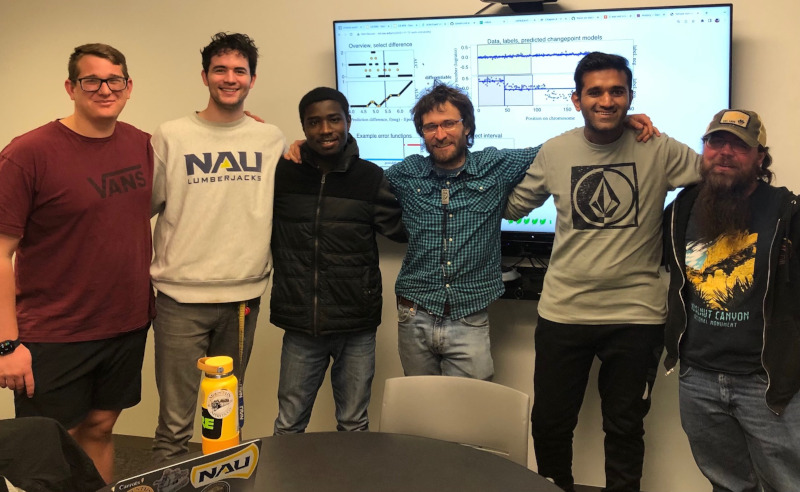
\includegraphics[height=5cm]{2023-02-02-group-meeting} \\
}

\date{}

\maketitle

\section{Problem Setting 1: ROC curves for evaluating supervised  binary classification algorithms}

\begin{frame}
  \frametitle{Problem: supervised binary classification}
  
  \begin{itemize}
  \item Given pairs of inputs $\mathbf x\in\mathbb R^p$ and outputs
    $y\in\{0,1\}$ can we learn a score 
    $f(\mathbf x)\in\mathbb R$, predict $y=1$ when $f(\mathbf x)>0$?
  \item Example: email, $\mathbf x =$bag of words, $y=$spam or not.
  \item Example: images. Jones {\it et al.} PNAS 2009.
    \parbox{2in}{\includegraphics[width=2in]{cellprofiler}}
    \parbox{1.9in}{Most algorithms (SVM, Logistic regression, etc) minimize a differentiable surrogate of zero-one loss = sum of:\\
      \textbf{False positives:} $f(\mathbf x)>0$ but $y=0$ (predict
      budding, but cell is not).\\
      \textbf{False negatives:} $f(\mathbf x)<0$ but $y=1$ (predict
      not budding, but cell is).  }
  \end{itemize} 
\end{frame}

\begin{frame}
  \frametitle{ROC curves for evaluation, especially useful with imbalance}

  \includegraphics[width=0.65\textwidth]{figure-batchtools-expired-earth-roc}

  \begin{itemize}
  \item At default FPR=24\% (D), glmnet has fewer errors.
  \item At FPR=4\%, xgboost has fewer errors.
  \end{itemize}
\end{frame}

\begin{frame}
  \frametitle{Receiver Operating Characteristic (ROC) Curves}
  \begin{itemize}
  \item Classic evaluation method from the signal processing
    literature (Egan and Egan, 1975).
  \item ROC curve of learned $f$ is plot of True
    Positive Rate vs False Positive Rate: each point on the ROC curve
    is a different constant $c\in\mathbb R$ added to the predicted
    values: $f(\mathbf x)+c$.
  \item $c=\infty$ means always predict positive label (FPR=TPR=1).
  \item $c=-\infty$ means always predict negative label (FPR=TPR=0).
  \item Best classifier has a point near upper left (TPR=1, FPR=0), with large
    Area Under the Curve (AUC).
  % \item Proposed idea: a new surrogate for AUC that is differentiable,
  %   so can be used for gradient descent learning.
  \end{itemize}
  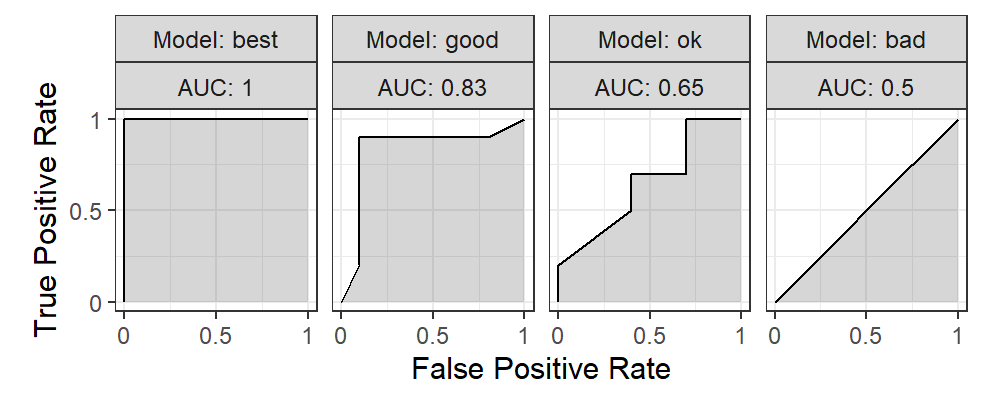
\includegraphics[width=0.9\textwidth]{figure-more-than-one-new-binary}
\end{frame}



\begin{frame}
  \frametitle{Research question and new idea}
  Can we learn a binary classification function $f$ which directly
  optimizes the ROC curve?
  \begin{itemize}
  \item Most algorithms involve minimizing a differentiable surrogate
    of the zero-one loss, which is not the same.
  \item The Area Under the ROC Curve (AUC) is piecewise constant
    (gradient zero almost everywhere), so can not be used with
    gradient descent algorithms.
  \item We proposed (Hocking, Hillman 2023) to encourage points to be in the upper left of ROC
    space, using a loss function which is a differentiable surrogate
    of the sum of min(FPR,FNR).
  \end{itemize}
  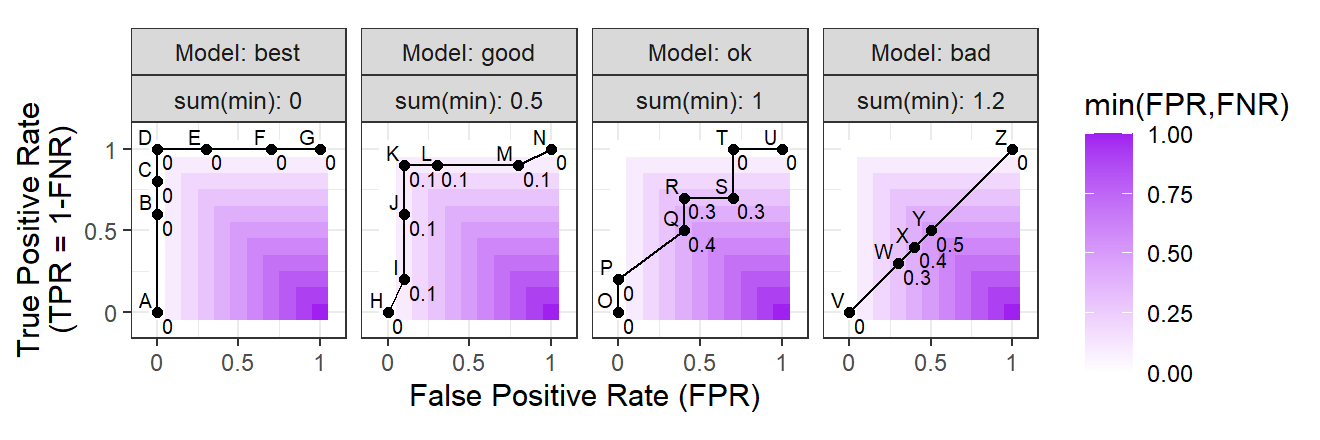
\includegraphics[width=\textwidth]{figure-more-than-one-new-binary-heat}
\end{frame}
 
\section{ROC curve optimization using sort-based gradient descent}

\begin{frame}
  \frametitle{Gradients of sample-based loss are influenced by imbalance}
  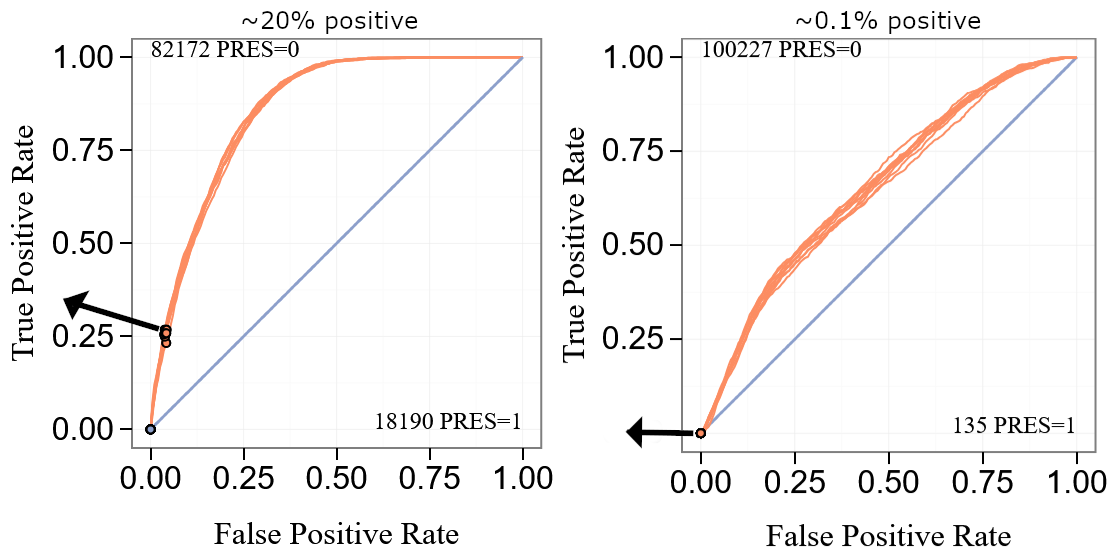
\includegraphics[width=\textwidth]{roc-gradient-arrows}
  \begin{itemize}
  \item Left: some imbalance, ~20\% positive labels, gradient 4x
    stronger along X axis / False Positive Rate.
  \item Right: large imbalance, ~0.1\% positive labels, gradient 1000x
    stronger along X axis / False Positive Rate. (True Positive / Y
    axis gradients essentially ignored)
  \end{itemize}
\end{frame}

\begin{frame}
  \frametitle{Gradients using balanced sample weights, proposed loss}
  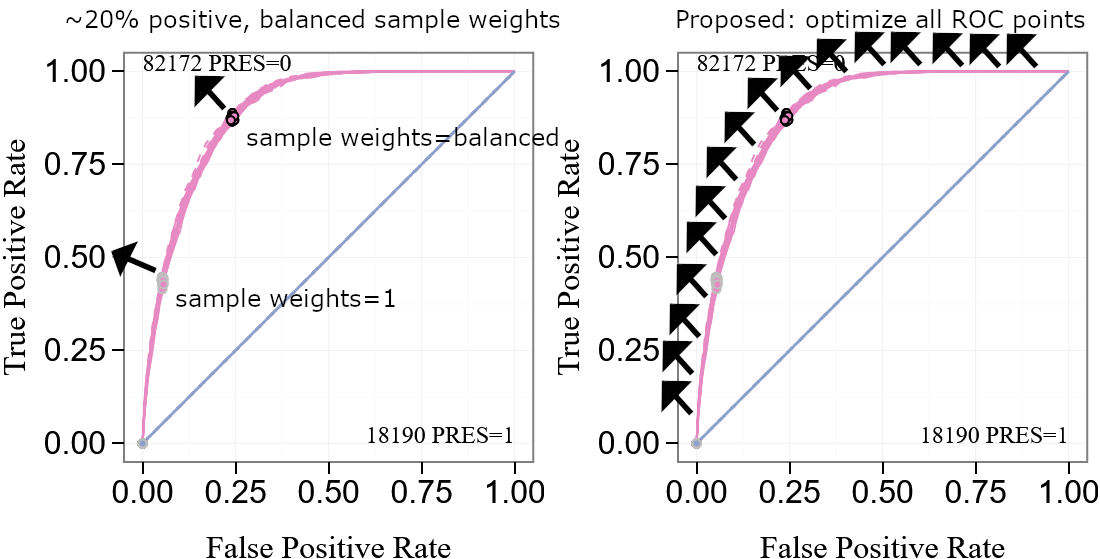
\includegraphics[width=\textwidth]{roc-gradient-arrows-proposed}
  \begin{itemize}
  \item Left: gradient 4x
    stronger along X axis for sample weights=1. Balanced sample
    weights mean equal influence for gradients along both axes, based on the current prediction threshold.
  \item Right: proposed method computes gradients based on all ROC
    points, not just the current prediction threshold.
  \end{itemize}
\end{frame}

\begin{frame}
  \frametitle{Comparing proposed loss with baselines}
  \begin{itemize}
  \small
  \item Classic baselines: hinge and logistic loss, sum over samples, $\ell[yf(x)]$.
  \item Bamber (1975) proved ROC-AUC relation to Mann-Whitney
    U statistic (double sum over all pairs of positive and negative
    samples).
  \item Recently:  $\text{SVM}^{\text{struct}}$ (Joachims 2005),
    X-risk (Yang 2022), %https://arxiv.org/abs/2206.00439
    All Pairs Squared Hinge (Rust and Hocking 2023),
    sum loss over pairs of positive and negative samples, $\ell[f(x^+)-f(x^-)]$.
  \item Proposed: sort-based AUM loss (sum over points on ROC curve).
  \item Figure below: loss for two samples: one positive, one negative.
  \end{itemize}

  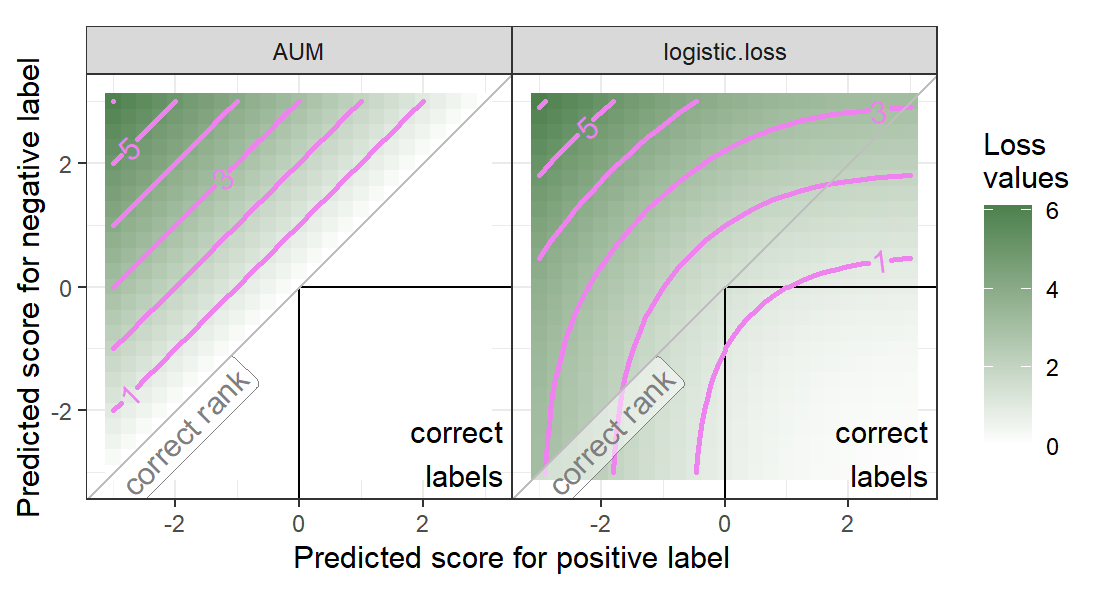
\includegraphics[width=0.7\textwidth]{figure-compare-hinge-loss-contours-logistic.png}

    Barr, Hocking, Morton, Thatcher, Shaw, \emph{TransAI} (2022).

  %AUM loss here = linear hinge with no margin, summed over pairs.
\end{frame}

\begin{frame}
  \frametitle{Large AUC $\approx$ small Area Under Min(FP,FN) (AUM)}
  \small
  
  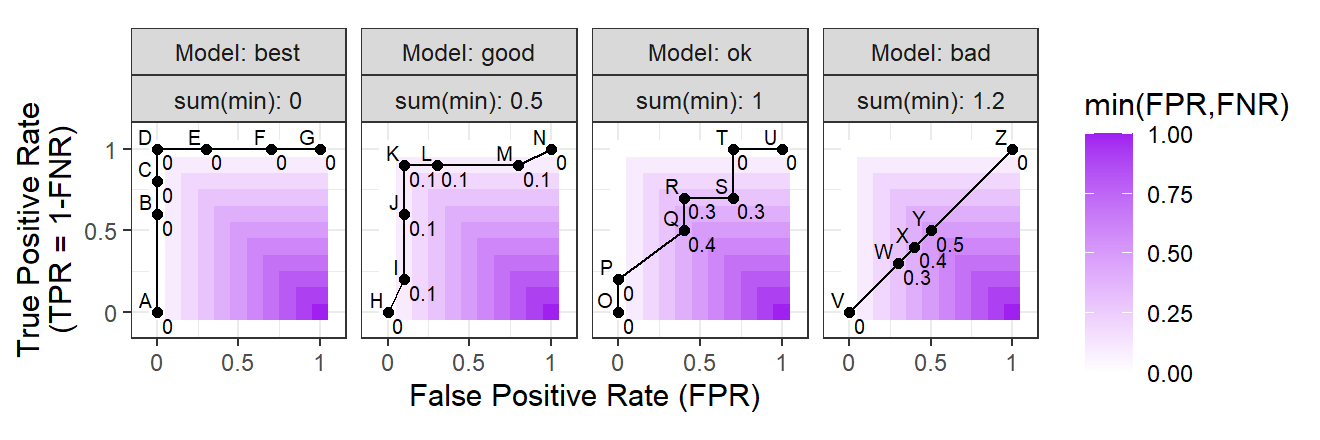
\includegraphics[height=1.3in]{figure-more-than-one-new-binary-heat}

  Above: purple heat map = numbers near dots = distance to top or left

  = same as black min error rate functions below.

  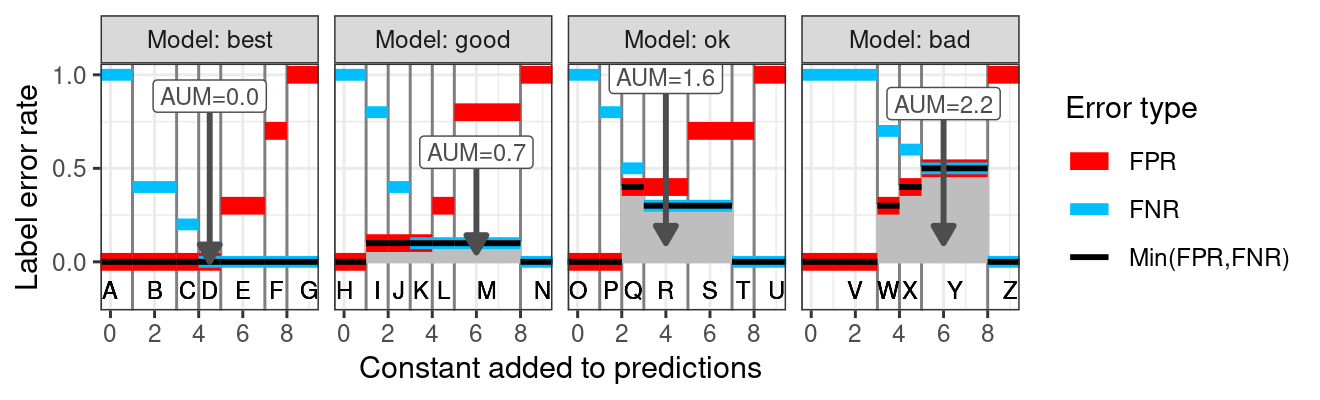
\includegraphics[height=1.3in]{figure-more-than-one-new-binary-aum-rate}

  Hocking, Hillman, \emph{Journal of Machine Learning Research} (2023).

  %Proposal: track how thresholds in error plot change with step size.
  
\end{frame}

\begin{frame}
  \frametitle{Computing Sum of Min (SM)}
  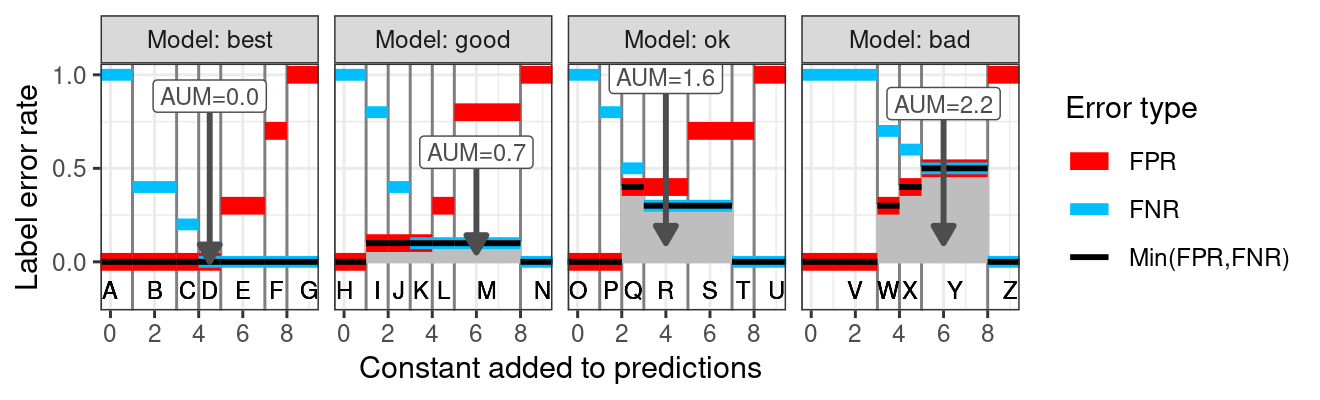
\includegraphics[width=\textwidth]{figure-more-than-one-new-binary-aum-rate}
  \vskip -0.2cm
  \begin{itemize}
  \item For $N$ samples, there are $\leq N+1$ points on the ROC curve,
  \item with sorted thresholds $T_1\leq\cdots\leq T_N\in\mathbb R$,
  \item and corresponding min error values $M_1,\dots,M_N$.
  \item Then if $I$ is the indicator function, we can write the sum of
    the min (SM), over all ROC points, as:
  \end{itemize}
\begin{equation*}
  \label{eq:SM-computation}
    \text{SM} =
    \sum_{i=2}^{N}
    I[ T_{i} \neq T_{i-1} ]
    M_i =
    \sum_{i:T_{i} \neq T_{i-1} }
    M_i.
\end{equation*}

($\neq$ required: a tie $T_i=T_{i-1}$ deletes a point from the ROC curve)

\end{frame}

\begin{frame}
  \frametitle{Computing Area Under Min (AUM)}
  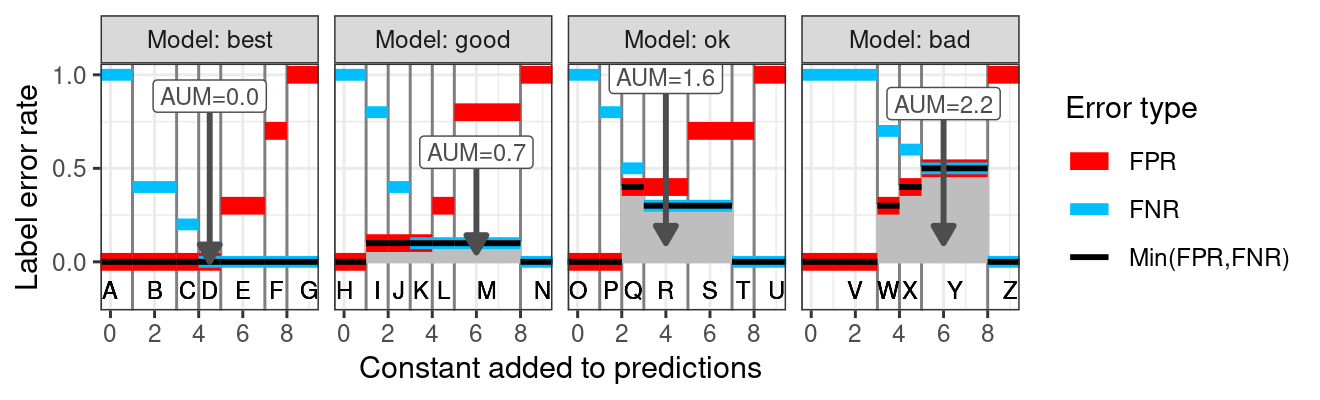
\includegraphics[width=\textwidth]{figure-more-than-one-new-binary-aum-rate}

The AUM can be interpreted as an L1 relaxation of SM,

\begin{eqnarray*}
    \text{SM} &=&
    \sum_{i=2}^{N}
    I[ T_{i} \neq T_{i-1} ]
    M_i =
    \sum_{i:T_{i} \neq T_{i-1} }
                  M_i.
                                    \\
    \text{AUM} &=&
    \sum_{i=2}^{N}
    [ T_{i} - T_{i-1} ]
                   M_i.\\
\end{eqnarray*}
AUM is therefore a surrogate loss for ROC optimization, and it is differentiable almost everywhere $\Rightarrow$ gradient descent learning!
\end{frame}

\begin{frame}[fragile]
  \frametitle{ROC curve pytorch code}
  \begin{verbatim}
def ROC_curve(pred_tensor, label_tensor):
    sorted_indices = torch.argsort(-pred_tensor)
    ...
    return { # a dictionary of torch tensors
        "FPR":FPR,
        "FNR":FNR,
        "TPR":1 - FNR,
        "min(FPR,FNR)":torch.minimum(FPR, FNR),
        "min_constant":torch.cat([
          torch.tensor([-torch.inf]), uniq_thresh]),
        "max_constant":torch.cat([
          uniq_thresh, torch.tensor([torch.inf])])
    }
\end{verbatim}

    \url{https://tdhock.github.io/blog/2024/torch-roc-aum/}

\end{frame}

\begin{frame}[fragile]
  \frametitle{AUC and AUM pytorch code uses argsort}

  \begin{itemize}
  \item ROC AUC and proposed AUM are both implemented by first
    computing the ROC curve.
  \end{itemize}
  \begin{verbatim}
def ROC_AUC(pred_tensor, label_tensor):
    roc = ROC_curve(pred_tensor, label_tensor)
    FPR_diff = roc["FPR"][1:]-roc["FPR"][:-1]
    TPR_sum = roc["TPR"][1:]+roc["TPR"][:-1]
    return torch.sum(FPR_diff*TPR_sum/2.0)

def Proposed_AUM(pred_tensor, label_tensor):
    roc = ROC_curve(pred_tensor, label_tensor)
    min_FPR_FNR = roc["min(FPR,FNR)"][1:-1]
    constant_diff = roc["min_constant"][1:].diff()
    return torch.sum(min_FPR_FNR * constant_diff)
\end{verbatim}

  \url{https://tdhock.github.io/blog/2024/torch-roc-aum/}
\end{frame}

\begin{frame}[fragile]
  \frametitle{AUM pytorch code, auto-grad demo}

  \begin{itemize}
  \item Assume two samples, $(x_0,y_0=0), (x_1,y_1=1)$,
  \item Plot objective and gradient with respect to predicted scores.
  \end{itemize}

  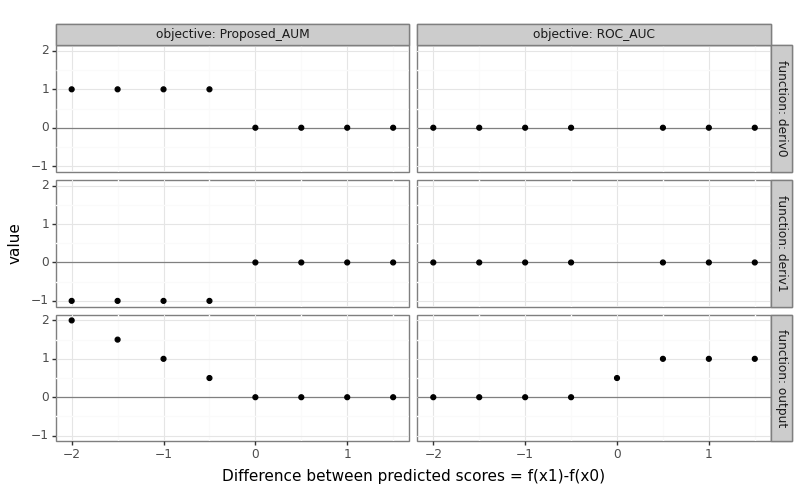
\includegraphics[width=\textwidth]{gg_aum_grad}

  \url{https://tdhock.github.io/blog/2024/torch-roc-aum/}
\end{frame}

\begin{frame}
  \frametitle{AUM gradient descent increases validation AUC,\\
    four image classification data sets}
 
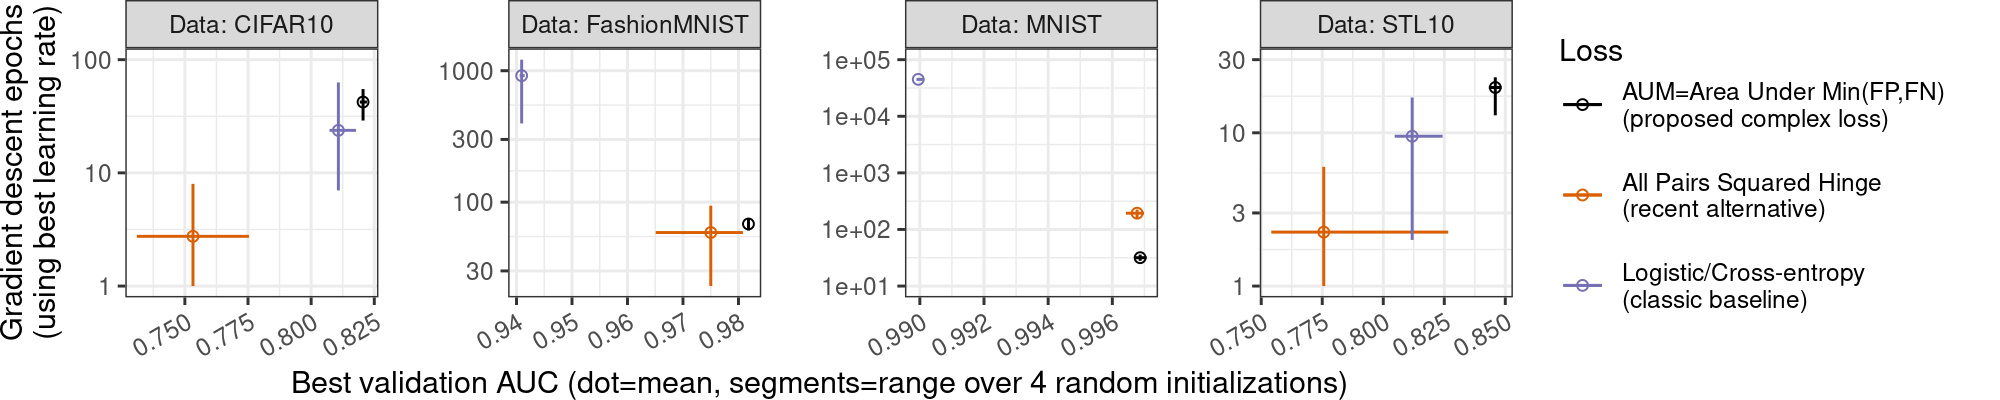
\includegraphics[width=\textwidth]{data_Classif_batchtools_best_valid_scatter}

\begin{itemize}
\item Implemented AUM loss using \texttt{torch.argsort} (auto-grad).
\item Gradient descent with constant step size, best of $10^{-4}$ to $10^5$.
\item Full gradient (batch size = number of samples).
\item Linear model, max iterations = 100,000.
\item Max Validation AUC comparable or better than baselines.
\item Number of epochs comparable to baselines.
\item Time per epoch is $O(N \log N)$ (sort), small log factor larger than standard logistic/cross-entropy loss, $O(N)$.
\end{itemize}

\end{frame}

\begin{frame}
  \frametitle{Discussion}
  \begin{itemize}
  \item Classic baselines are simple (sum over samples).
  \item Proposed AUM loss similar to recent losses that sum over all
    pairs of positive and negative examples (both can be implemented
    by sorting predicted scores); proposed AUM loss uses a
    different/novel relaxation.
  \item Proposed AUM loss implemented in 15 lines of pytorch code, can be used as a drop-in replacement for logistic/binary cross-entropy loss, \url{https://tdhock.github.io/blog/2024/torch-roc-aum/}
  \item Best use with stochastic gradient algorithms?
    At least one positive and one negative example is required in each
    batch.
  \item Margin-based algorithms like SVM?
  \item Works well in binary classification, how to adapt to
    multi-class setting, or other problems such as ranking/information
    retrieval? (next: change-point detection)
  \end{itemize}
\end{frame}

% \begin{frame}
%   \frametitle{TODO other classification data sets}
%  \includegraphics[width=\textwidth]{figure-unbalanced-grad-desc}
% \begin{itemize}
% \item TODO from JMLR paper
% \end{itemize}
% \end{frame}

\section{Problem setting 2: ROC curves for evaluating supervised changepoint algorithms}

\begin{frame}
  \frametitle{Problem: unsupervised changepoint detection}
  \begin{itemize}
  \item Data sequence $z_1,\dots,z_T$ at $T$ points over time/space.
  \item Ex: DNA copy number data for cancer diagnosis, $z_t\in\mathbb R$.
  \item The penalized changepoint problem (Maidstone \emph{et al.} 2017)
$$\argmin_{u_1,\dots,u_T\in\mathbb R} \sum_{t=1}^T (u_t - z_t)^2 + \lambda\sum_{t=2}^T I[u_{t-1} \neq u_t].$$
  \end{itemize}

  \parbox{0.6\textwidth}{
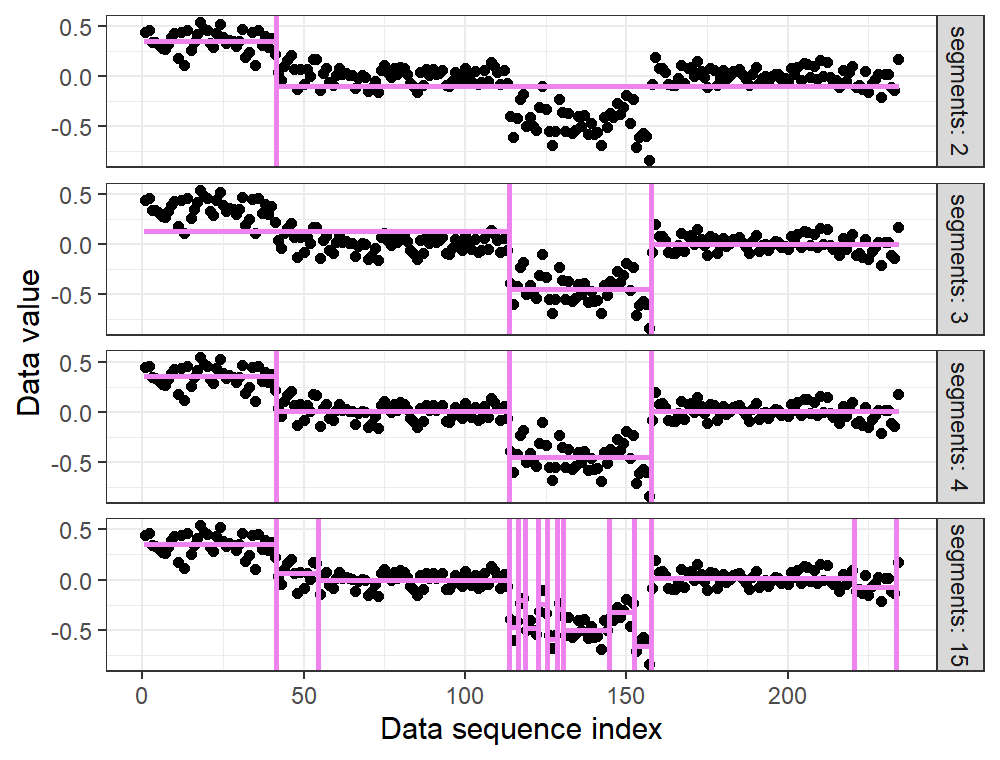
\includegraphics[width=0.6\textwidth]{figure-fn-not-monotonic-no-labels}
}
\parbox{0.3\textwidth}{
  Larger penalty $\lambda$ results in fewer changes/segments.

  \vskip 0.5in

  Smaller penalty $\lambda$ results in more changes/segments.
}

\end{frame}


\begin{frame}
  \frametitle{Problem: weakly supervised changepoint detection}
  \begin{itemize}
  \item First described by Hocking \emph{et al.} ICML 2013.
  \item We are given a data sequence $\mathbf z$ with labeled regions
    $L$.
  \end{itemize}

  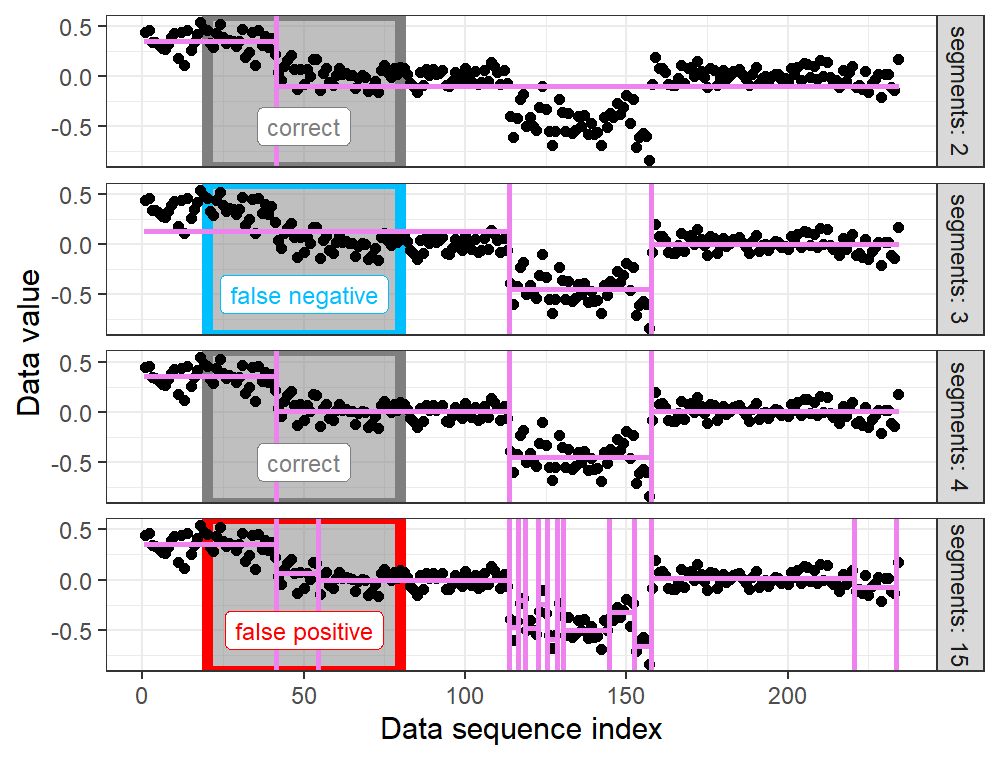
\includegraphics[width=0.56\textwidth]{figure-fn-not-monotonic}
  \only<2>{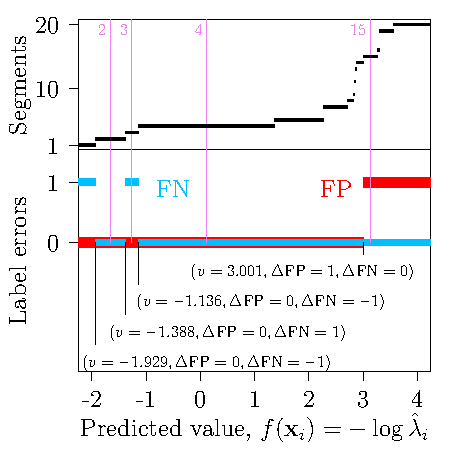
\includegraphics[width=0.42\textwidth]{figure-fn-not-monotonic-error-standAlone}}

  \only<2>{We compute features $\mathbf x=\phi(\mathbf z)\in\mathbf R^p$
    and want to learn a function $f(\mathbf x)=-\log\lambda\in\mathbf R$ that minimizes label error (sum of false positives and false negatives), or maximizes AUC, Hocking, Hillman, \emph{Journal of Machine Learning Research} (2023).}

\end{frame}

\begin{frame}
  \frametitle{Comparing changepoint algorithms using ROC curves}
  Hocking TD, Srivastava A. Labeled Optimal
  Partitioning. Computational Statistics (2022).
  
  \includegraphics[width=0.8\textwidth]{figure-LOPART-roc}

  LOPART algorithm (R package LOPART) has consistently larger
  test AUC than previous algorithms.
\end{frame}

\begin{frame}
  \frametitle{AUM gradient descent results in increased train AUC for
    a real changepoint problem}
 
Hillman, Hocking, \emph{Journal of Machine Learning Research} (2023).

\includegraphics[height=3.7cm]{figure-aum-optimized-iterations.png}
\includegraphics[height=3.7cm]{figure-aum-train-both.png}

\begin{itemize}
\item Left/middle: changepoint problem initialized to prediction vector with
  min label errors, gradient descent on prediction vector.
\item Right: linear model initialized by minimizing regularized convex
  loss (surrogate for label error, Hocking \emph{et al.} ICML 2013),
  gradient descent on weight vector.
\end{itemize}

\end{frame}

\section{Proposed complete line search algorithm for surrogate loss: Area Under Min\{FP,FN\} (AUM)} 

\begin{frame}
  \frametitle{Using thresholds to compute AUM}
  % \begin{itemize}
  % \item $n$ is the number of observations (labeled examples or sequences),
  % \item $B$ is the number of breakpoints in label error functions,
  % \item each breakpoint $b\in\{1,\dots, B\}$ is represented by the tuple $(v_b, \Delta\text{FP}_b, \Delta\text{FN}_b, \mathcal I_b)$,
  % \item $\mathcal I_b\in\{1,\dots,n\}$ is an example index, so there are changes $\Delta\text{FP}_b, \Delta\text{FN}_b$ at predicted value $v_b\in\mathbb R$ in the error functions
  % \end{itemize}
  % Let 
  % let $p_1,\dots,p_B$ be a permutation of $1,\dots,B$ such that
  % thresholds are increasing: $T_$
Hillman and Hocking, JMLR 2023, showed that AUM for the
current predictions, can be computed efficiently, as a function of
$T_1<\cdots<T_B$, thresholds when min label error $M_b$ changes,
\begin{equation*}
  \text{AUM} = \sum_{b=2}^B [T_{b} - T_{b-1}] M_b
\end{equation*}

This contribution: when learning a linear model,
$f(\mathbf x)= \mathbf w^T \mathbf x$, we can update the weights
$\mathbf w$ using AUM gradient descent. We compute an exact
representation of thresholds $T_b(s)$ and min error $M_b(s)$ as a
function of step size $s$, which results in a complete piecewise
linear representation of
\begin{equation*}
  \text{AUM}(s) = \sum_{b=2}^B [T_{b}(s) - T_{b-1}(s)] M_b(s).
\end{equation*}
 
\end{frame}

\begin{frame}
\frametitle{Simple example, proposed line search with 4 binary labels}

  Theorem: when learning a linear model, $f(\mathbf x)= \mathbf w^T \mathbf x$,
  \begin{itemize}
  \item AUC is piecewise constant, and
  \item AUM is piecewise linear,
  \end{itemize}
  as a function of step size in gradient descent.

  \begin{center}
\parbox{0.6\textwidth}{
\hspace{0.0cm}
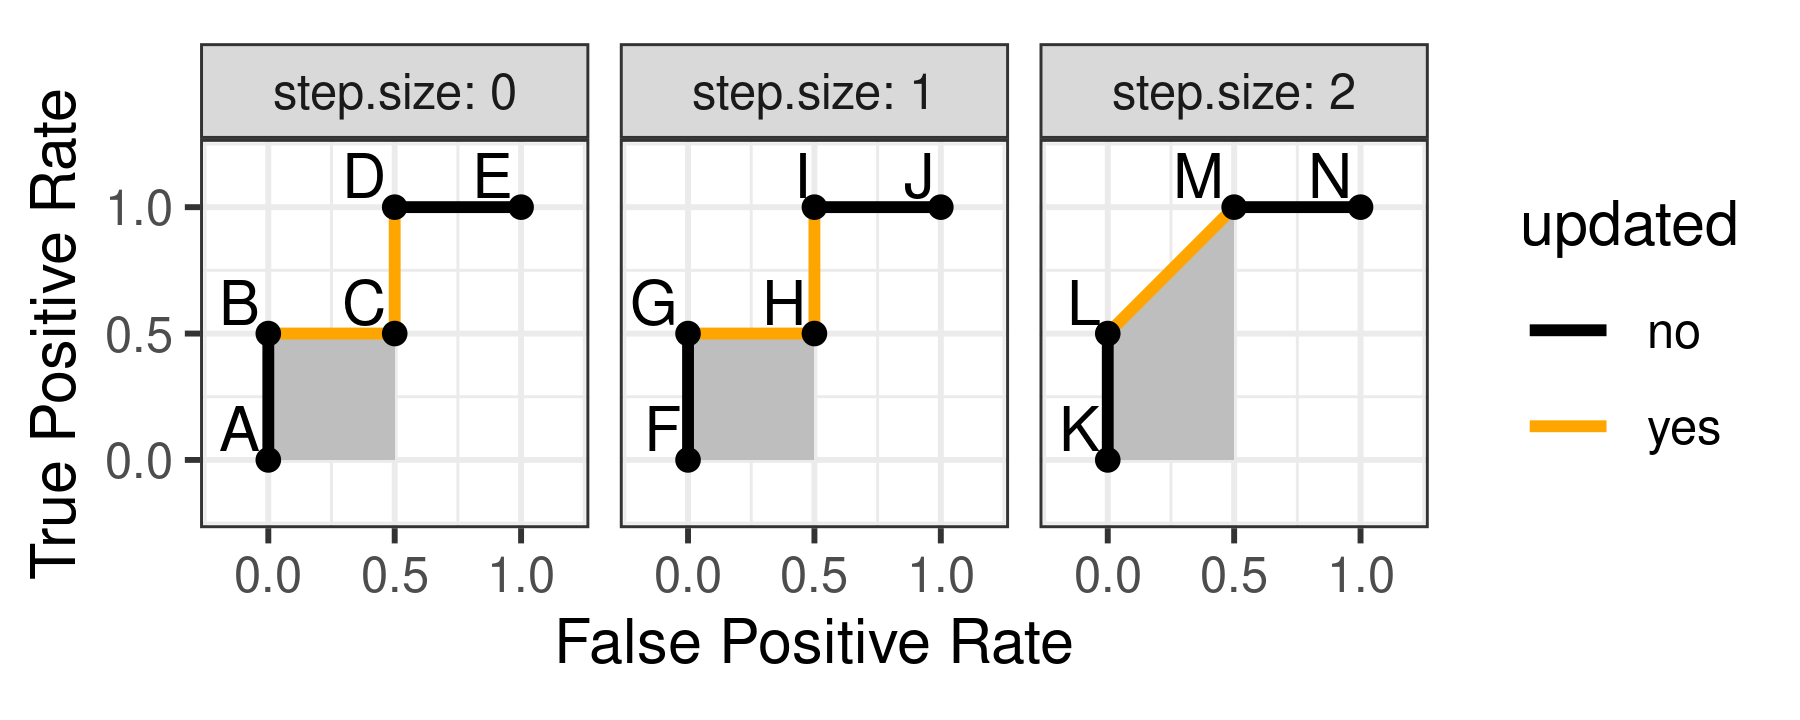
\includegraphics[width=0.5\textwidth]{figure-line-search-example-binary-roc.png}
\\
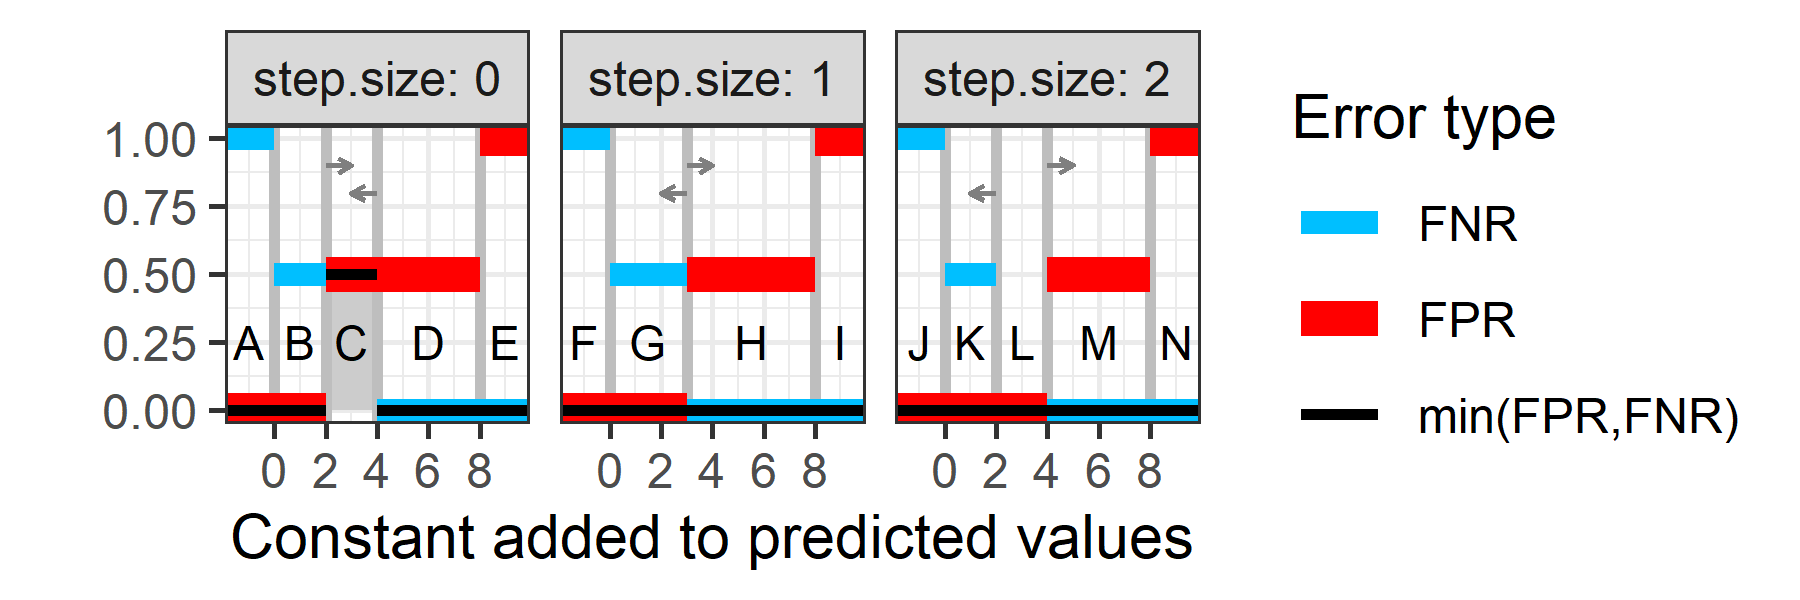
\includegraphics[width=0.6\textwidth]{figure-line-search-example-binary-error.png}\\
ROC curves and error functions
}\parbox{0.39\textwidth}{
  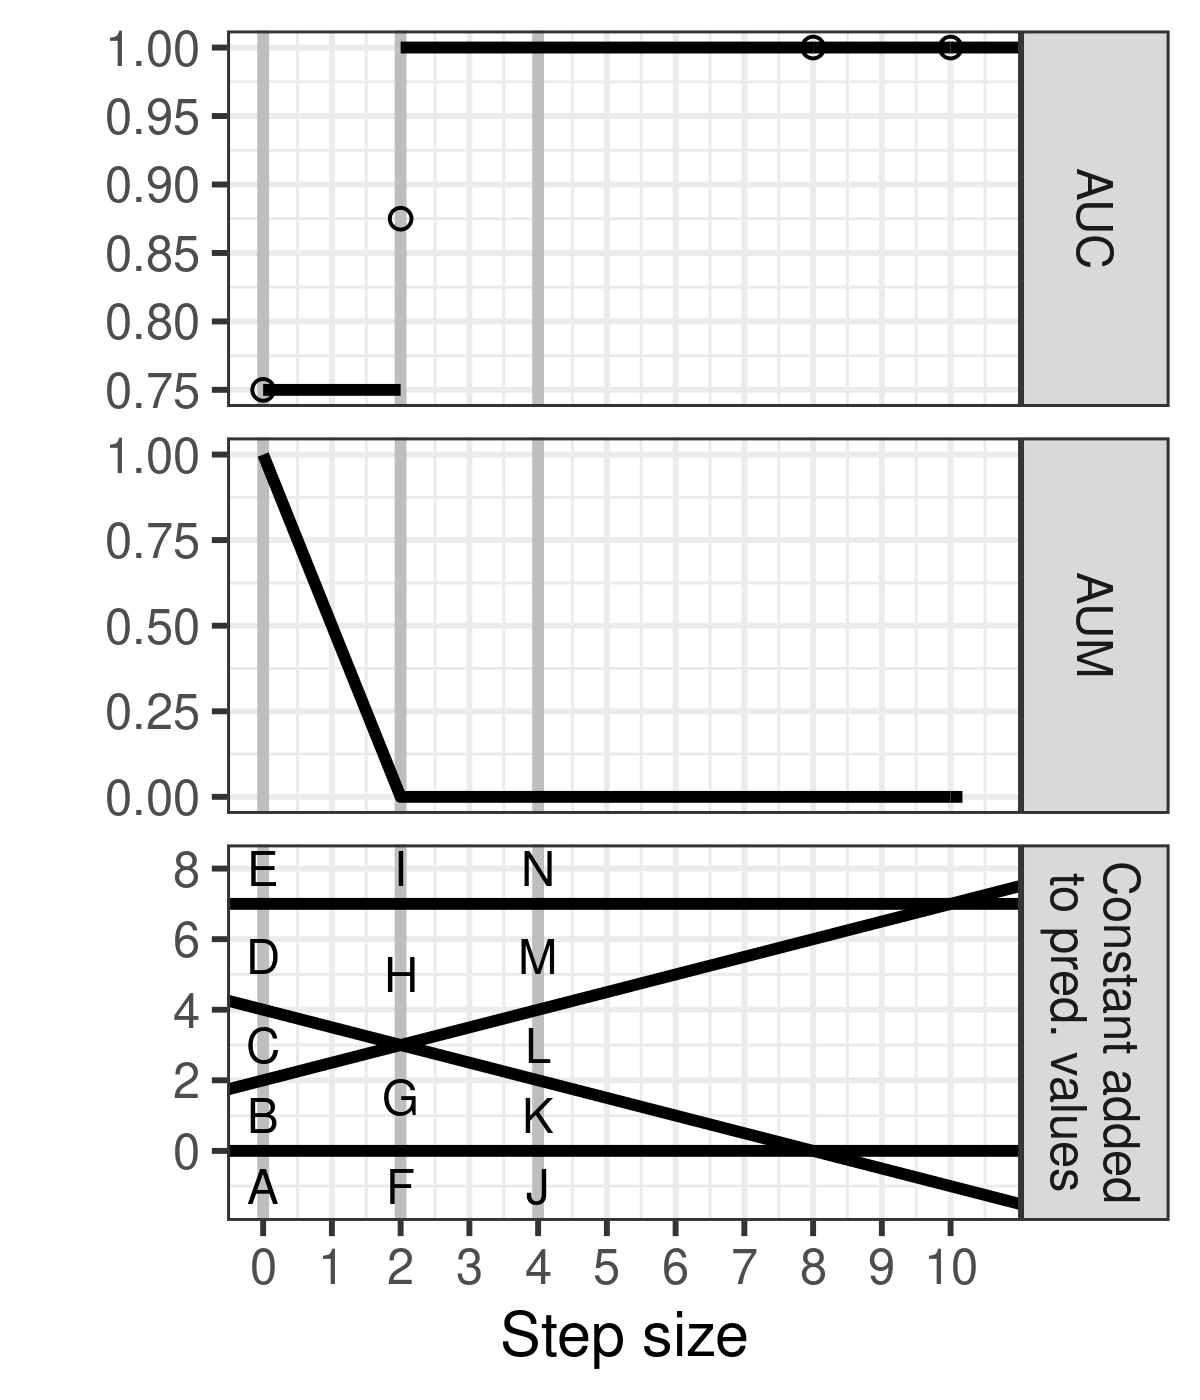
\includegraphics[width=0.35\textwidth]{figure-line-search-example-binary.png}\\
  Proposed line search
}
  \end{center}
  
  Letters show correspondence between points on the ROC curve, and intervals of constants added to predicted values.

\end{frame}


\begin{frame}
  \frametitle{Change-point example, comparison with grid search}

  Theorem: when learning a linear model, $f(\mathbf x)= \mathbf w^T \mathbf x$,
  \begin{itemize}
  \item AUC is piecewise constant, and
  \item AUM is piecewise linear,
  \end{itemize}
  as a function of step size in gradient descent.
  
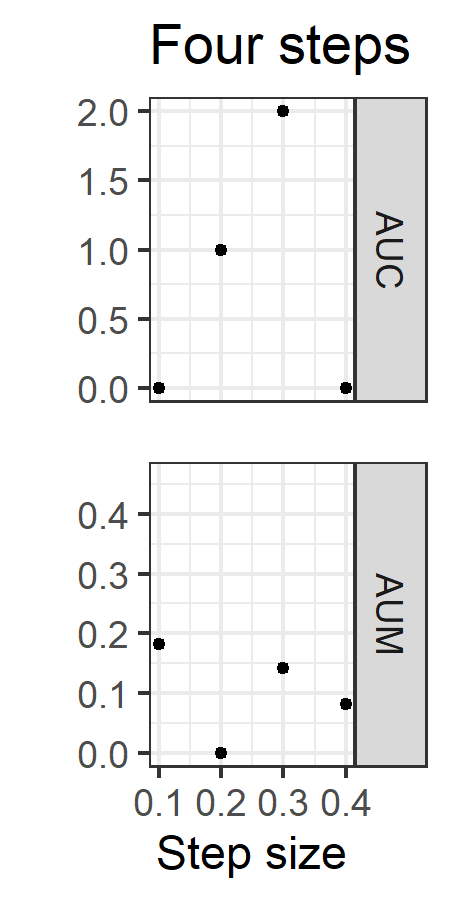
\includegraphics[height=5cm]{figure-line-search-example-some}
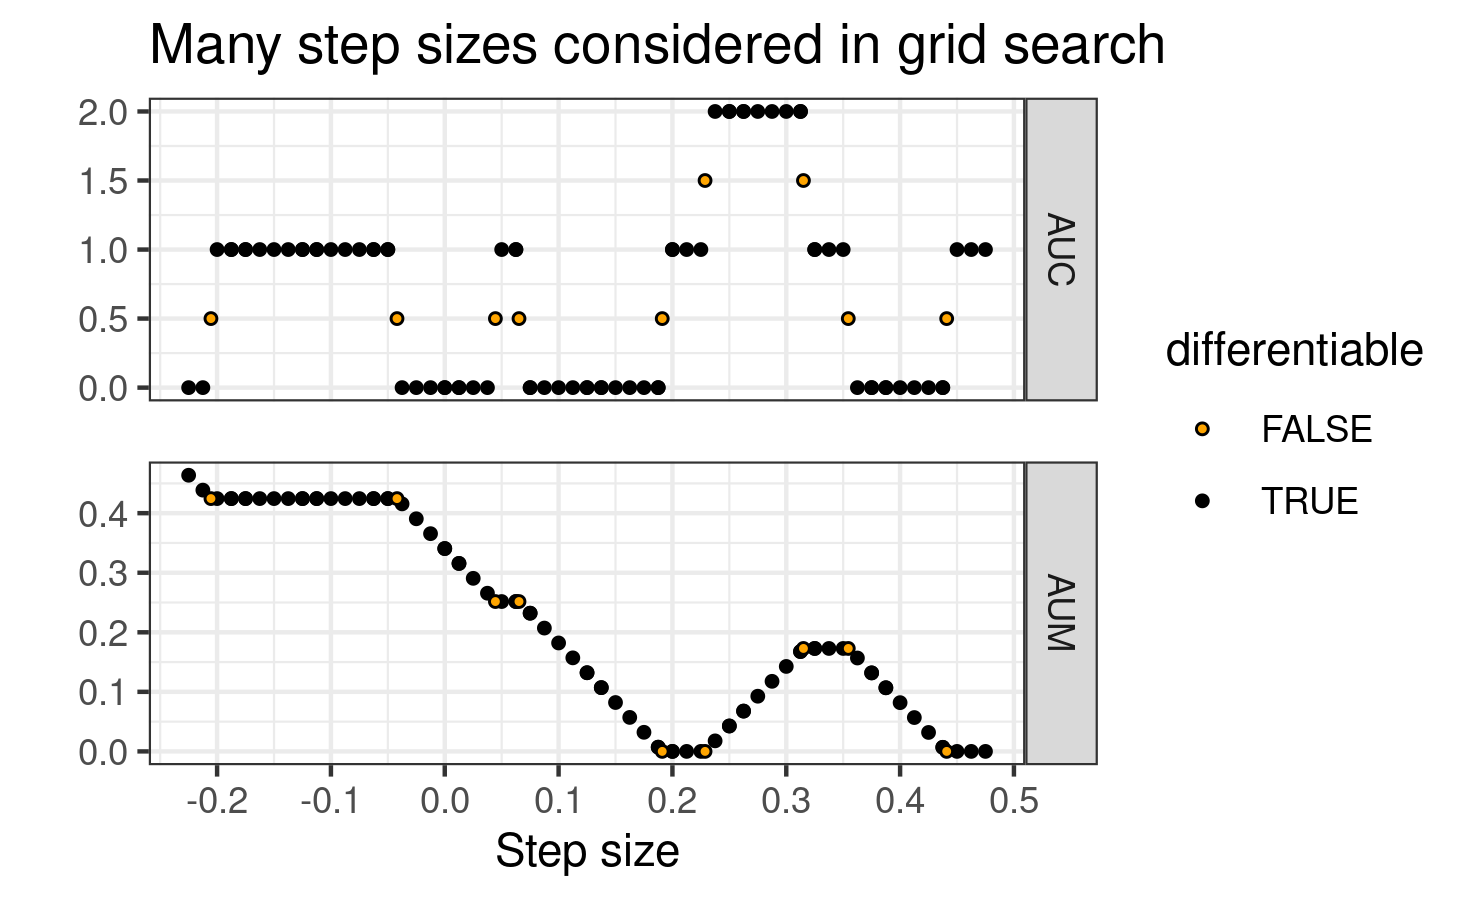
\includegraphics[height=5cm]{figure-line-search-example-grid}
 
Proposed line search algorithm computes updates when there are
possible changes in slope of AUM / values of AUC (orange dots).

\end{frame}


\begin{frame}
  \frametitle{AUM/AUC line search, iteration 1}
  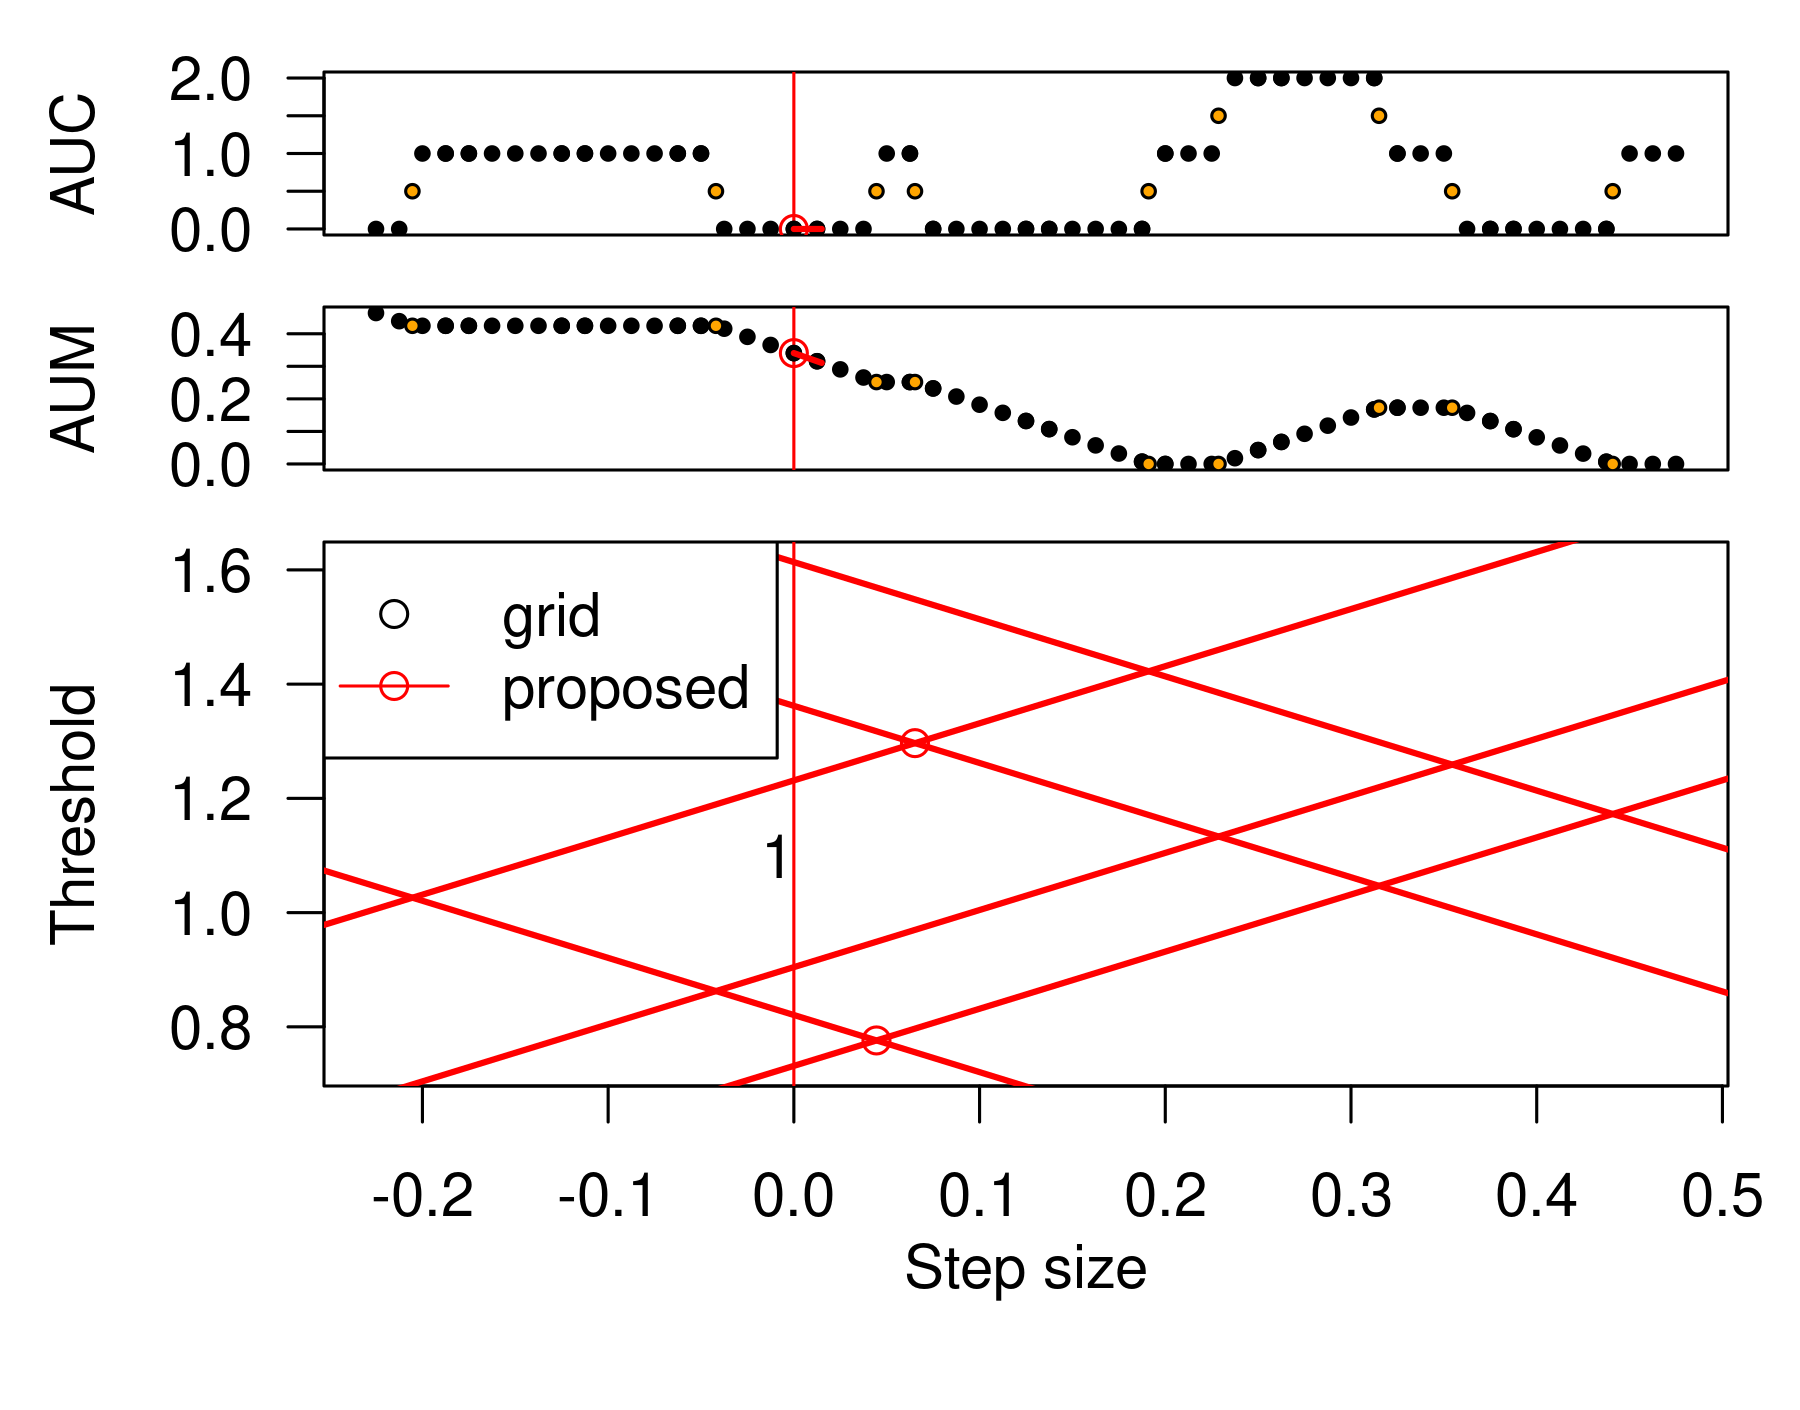
\includegraphics[width=\textwidth]{figure-line-search-example-1}
\end{frame}


\begin{frame}
  \frametitle{AUM/AUC line search, iteration 2}
  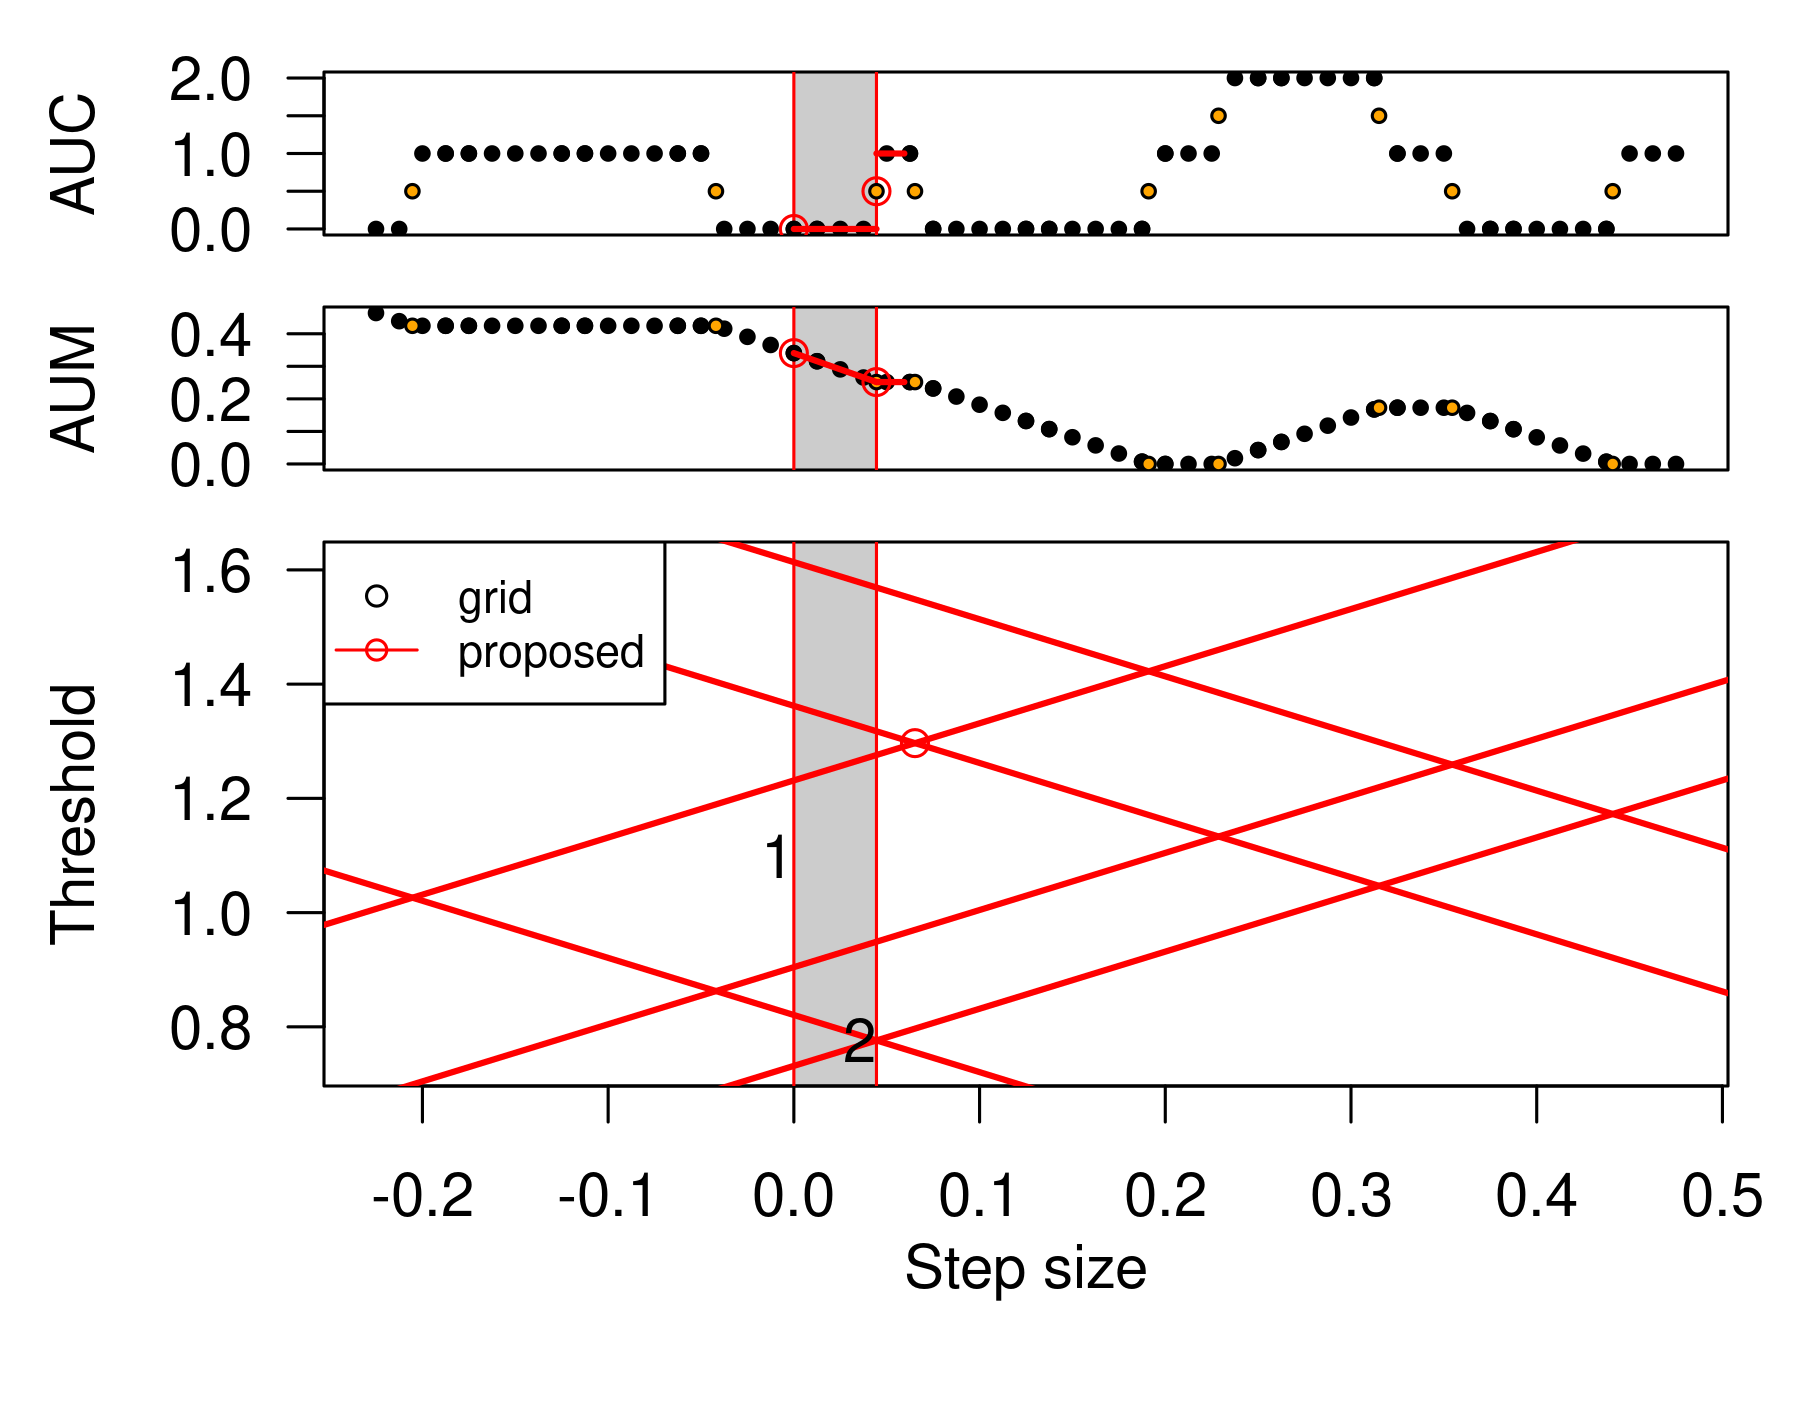
\includegraphics[width=\textwidth]{figure-line-search-example-2}
\end{frame}


\begin{frame}
  \frametitle{AUM/AUC line search, iteration 3}
  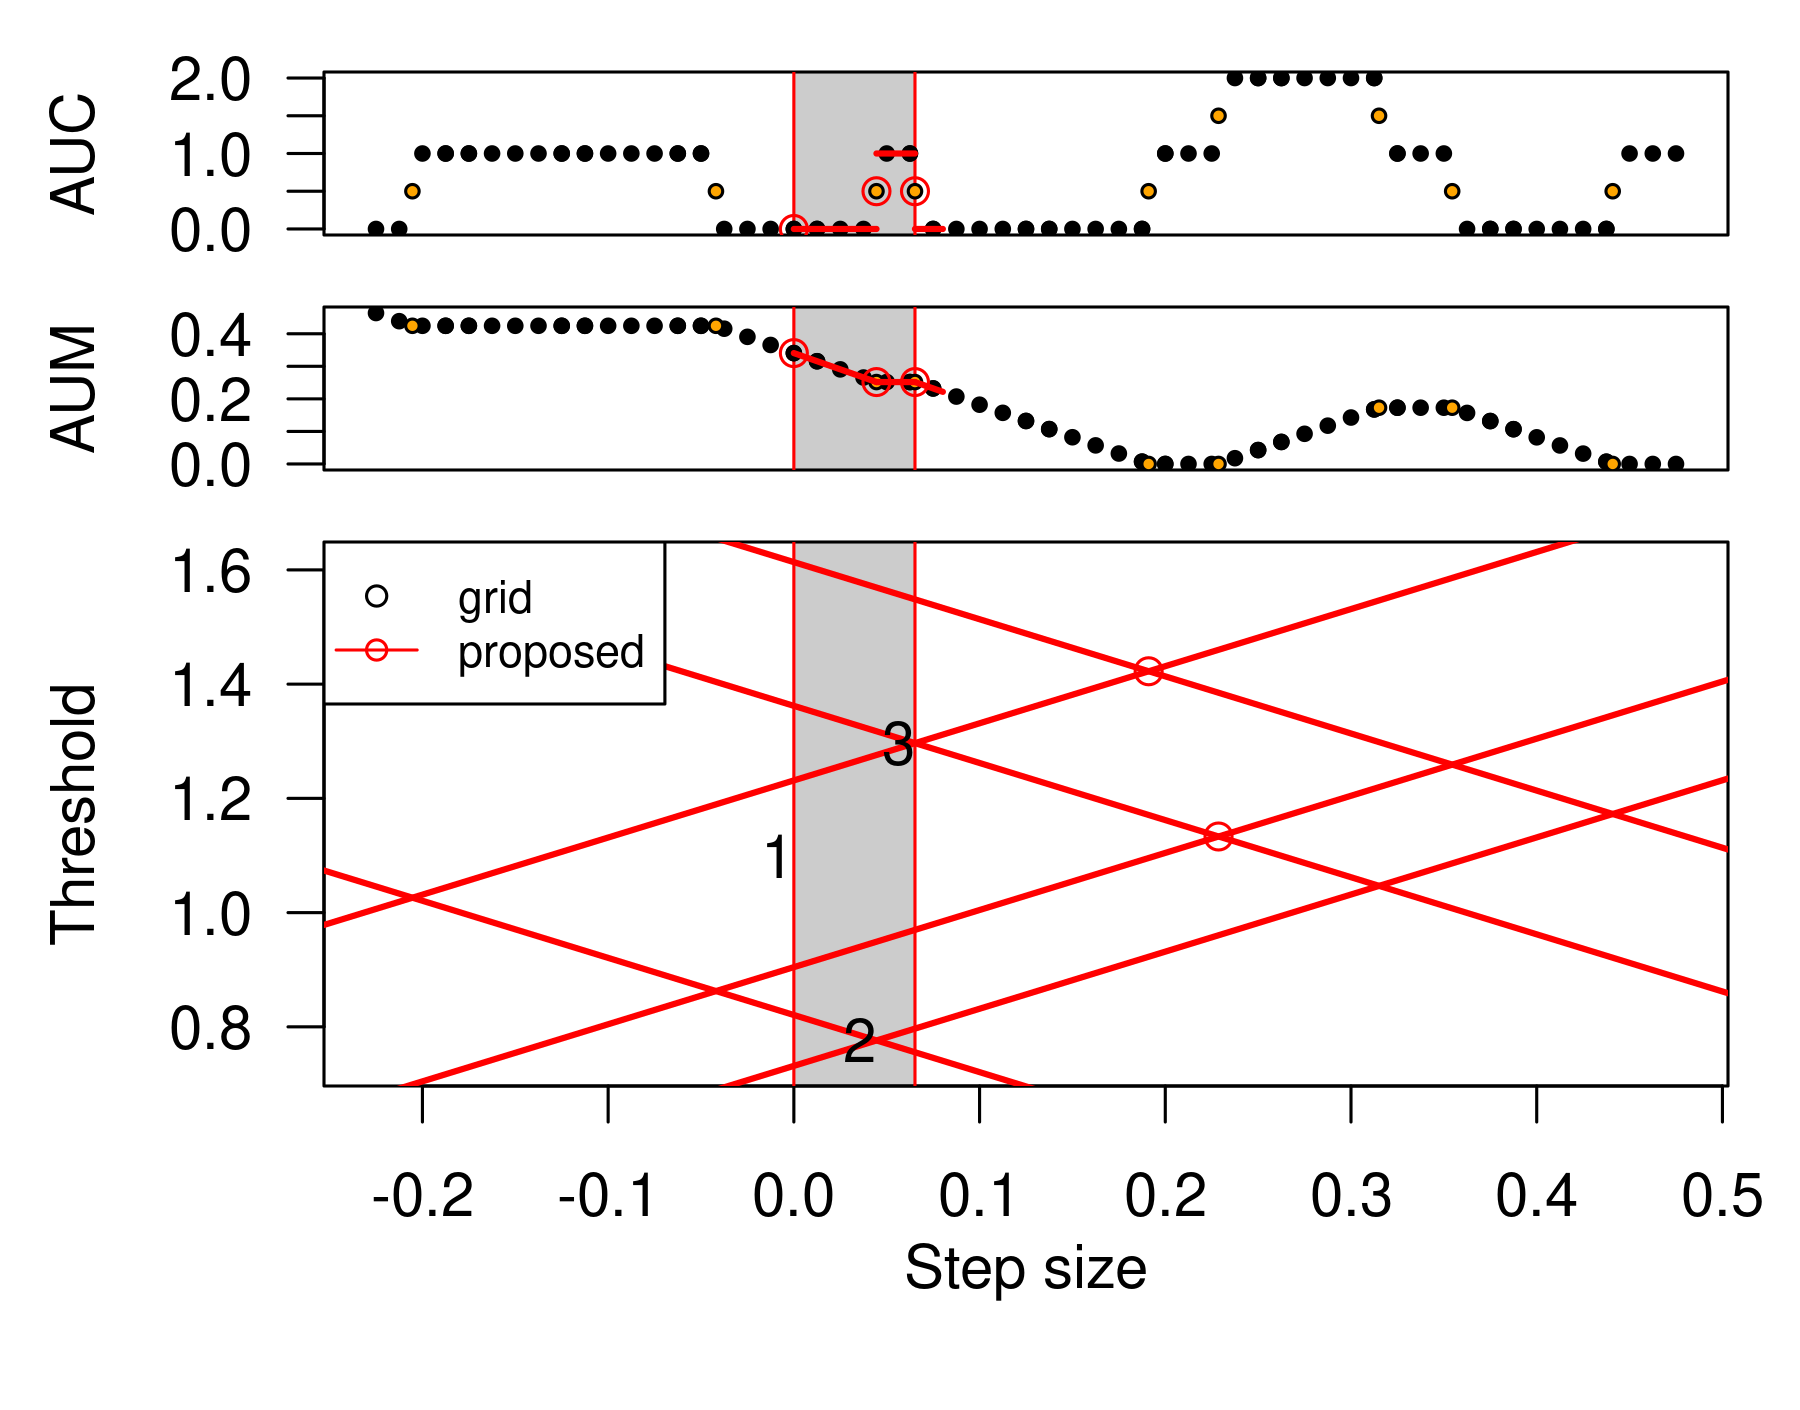
\includegraphics[width=\textwidth]{figure-line-search-example-3}
\end{frame}


\begin{frame}
  \frametitle{AUM/AUC line search, iteration 4}
  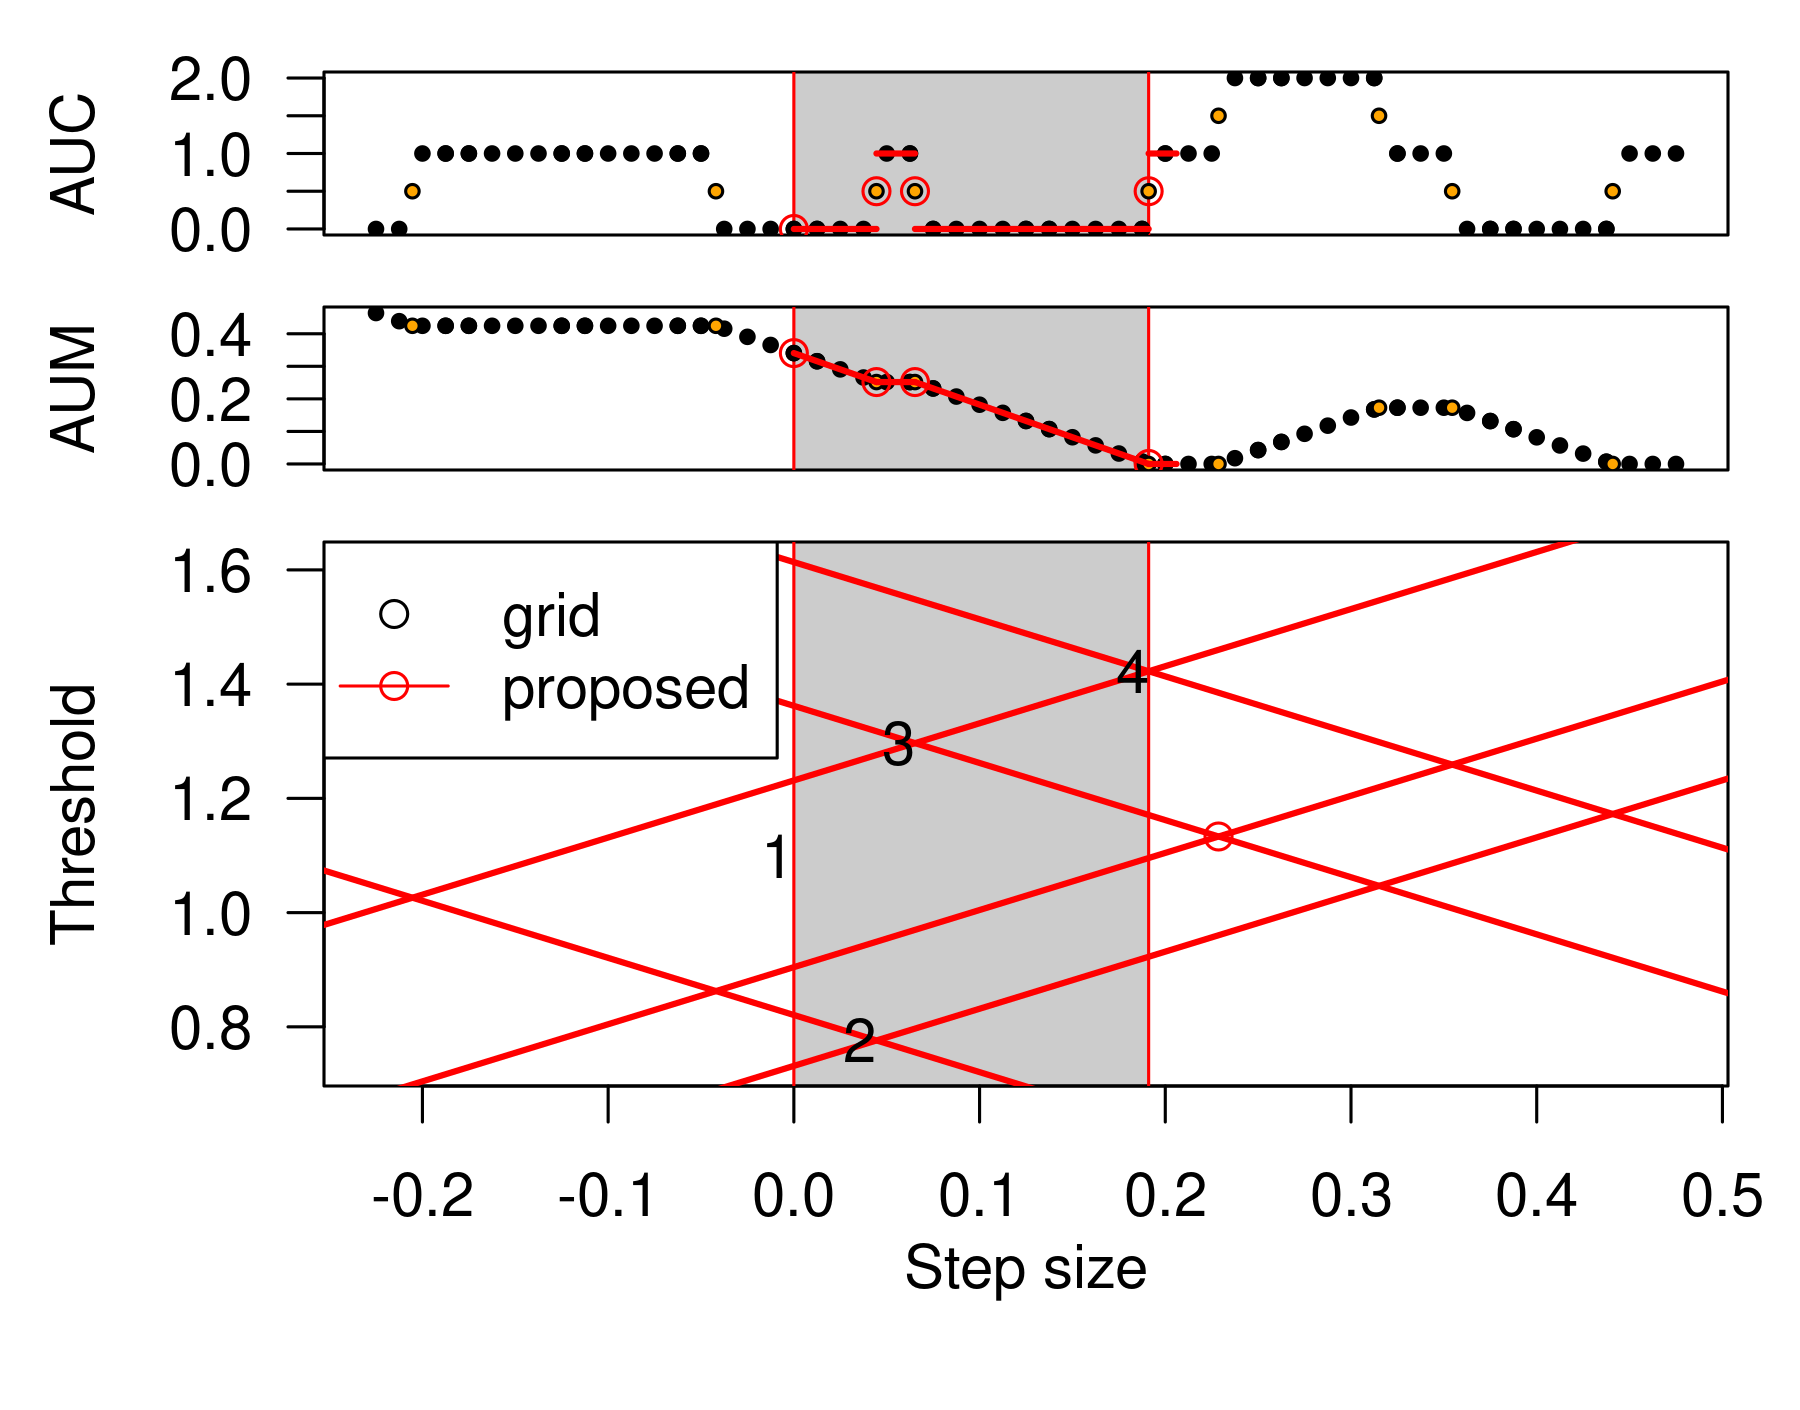
\includegraphics[width=\textwidth]{figure-line-search-example-4}
\end{frame}


\begin{frame}
  \frametitle{AUM/AUC line search, iteration 5}
  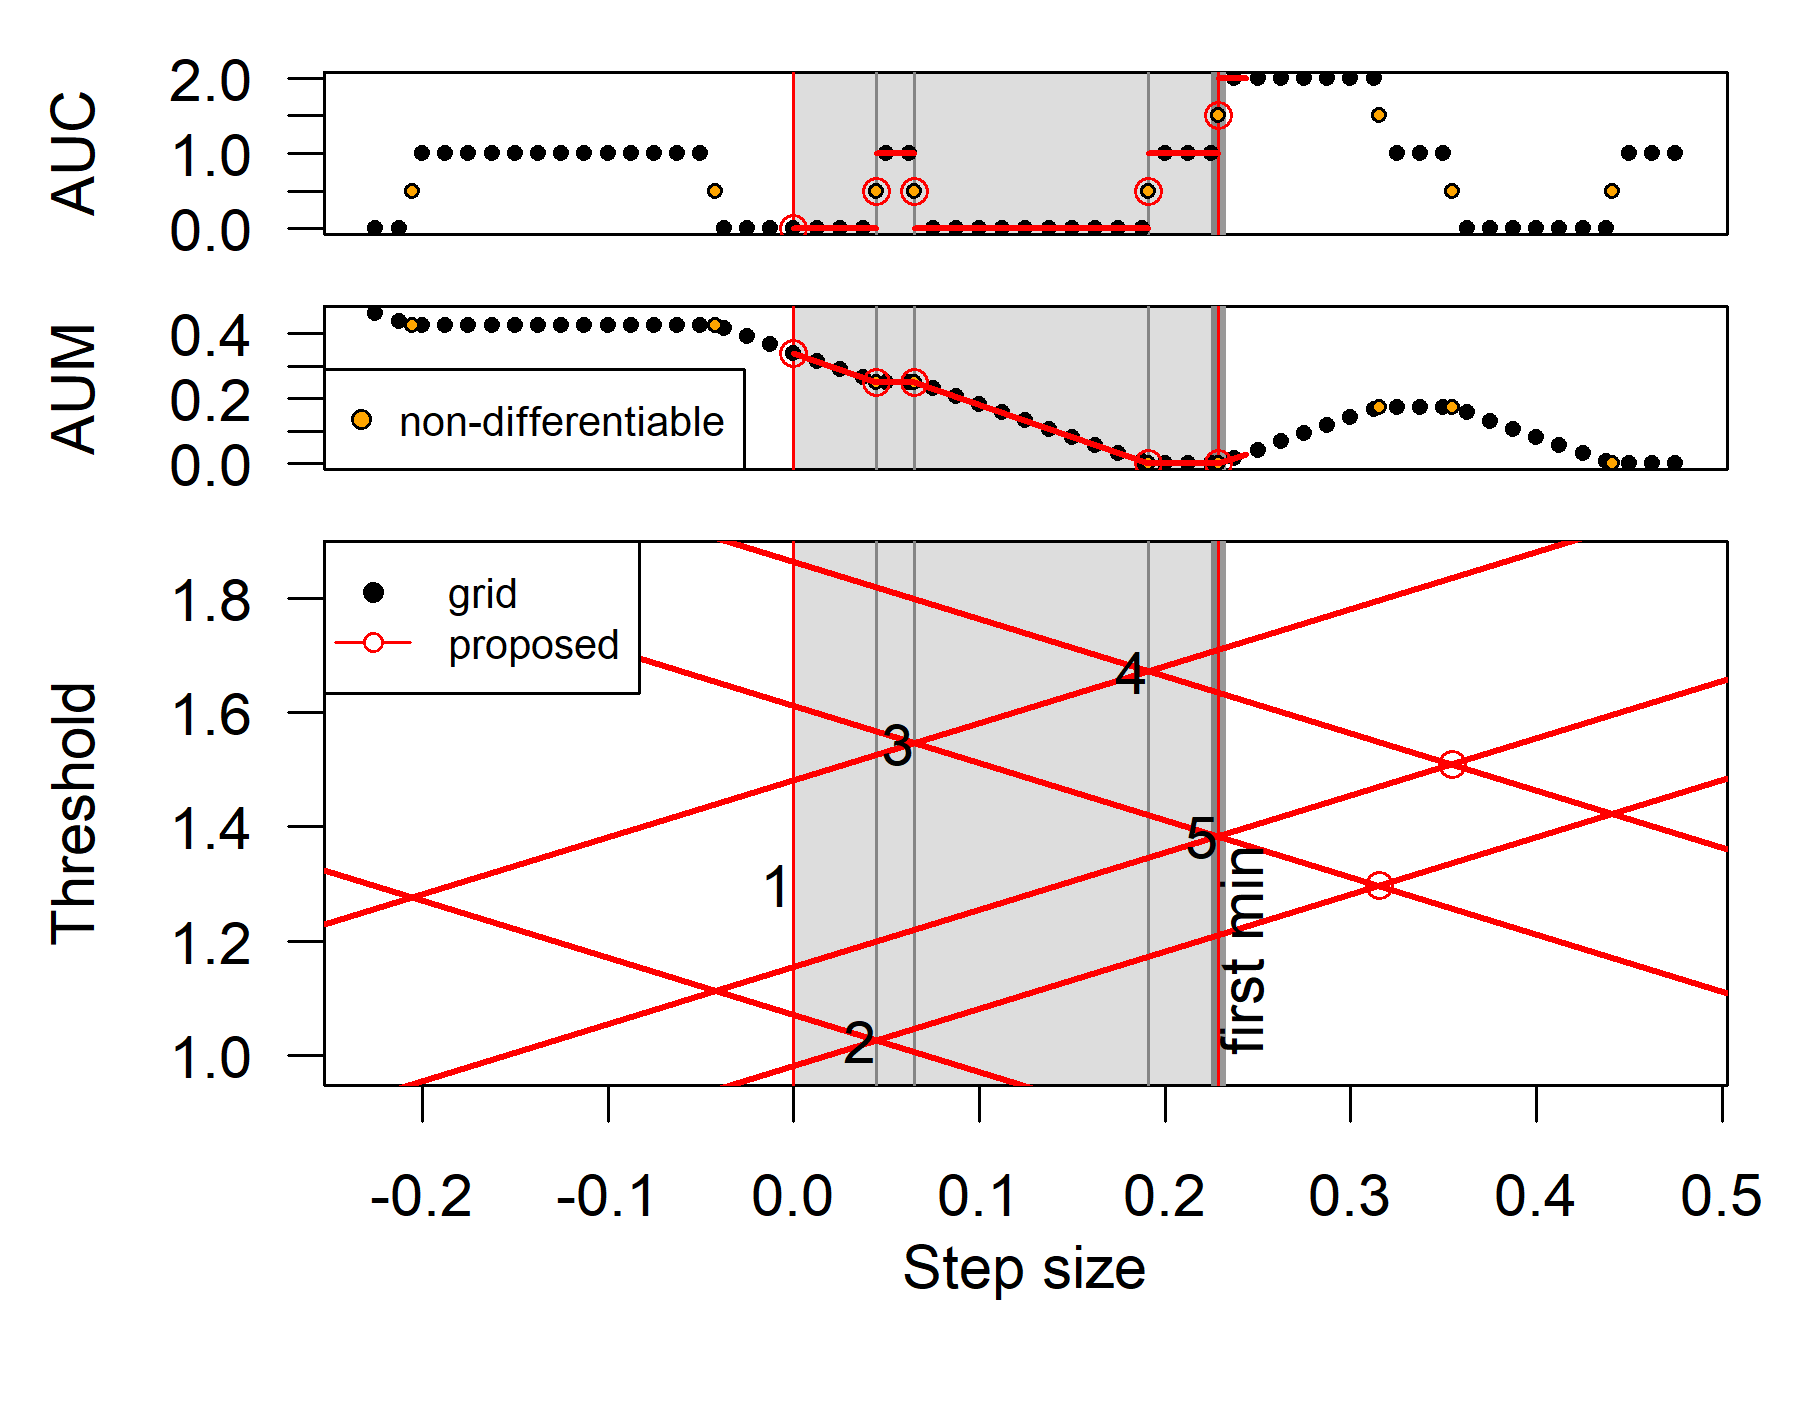
\includegraphics[width=\textwidth]{figure-line-search-example-5}
\end{frame}


\begin{frame}
  \frametitle{AUM/AUC line search, iteration 6}
  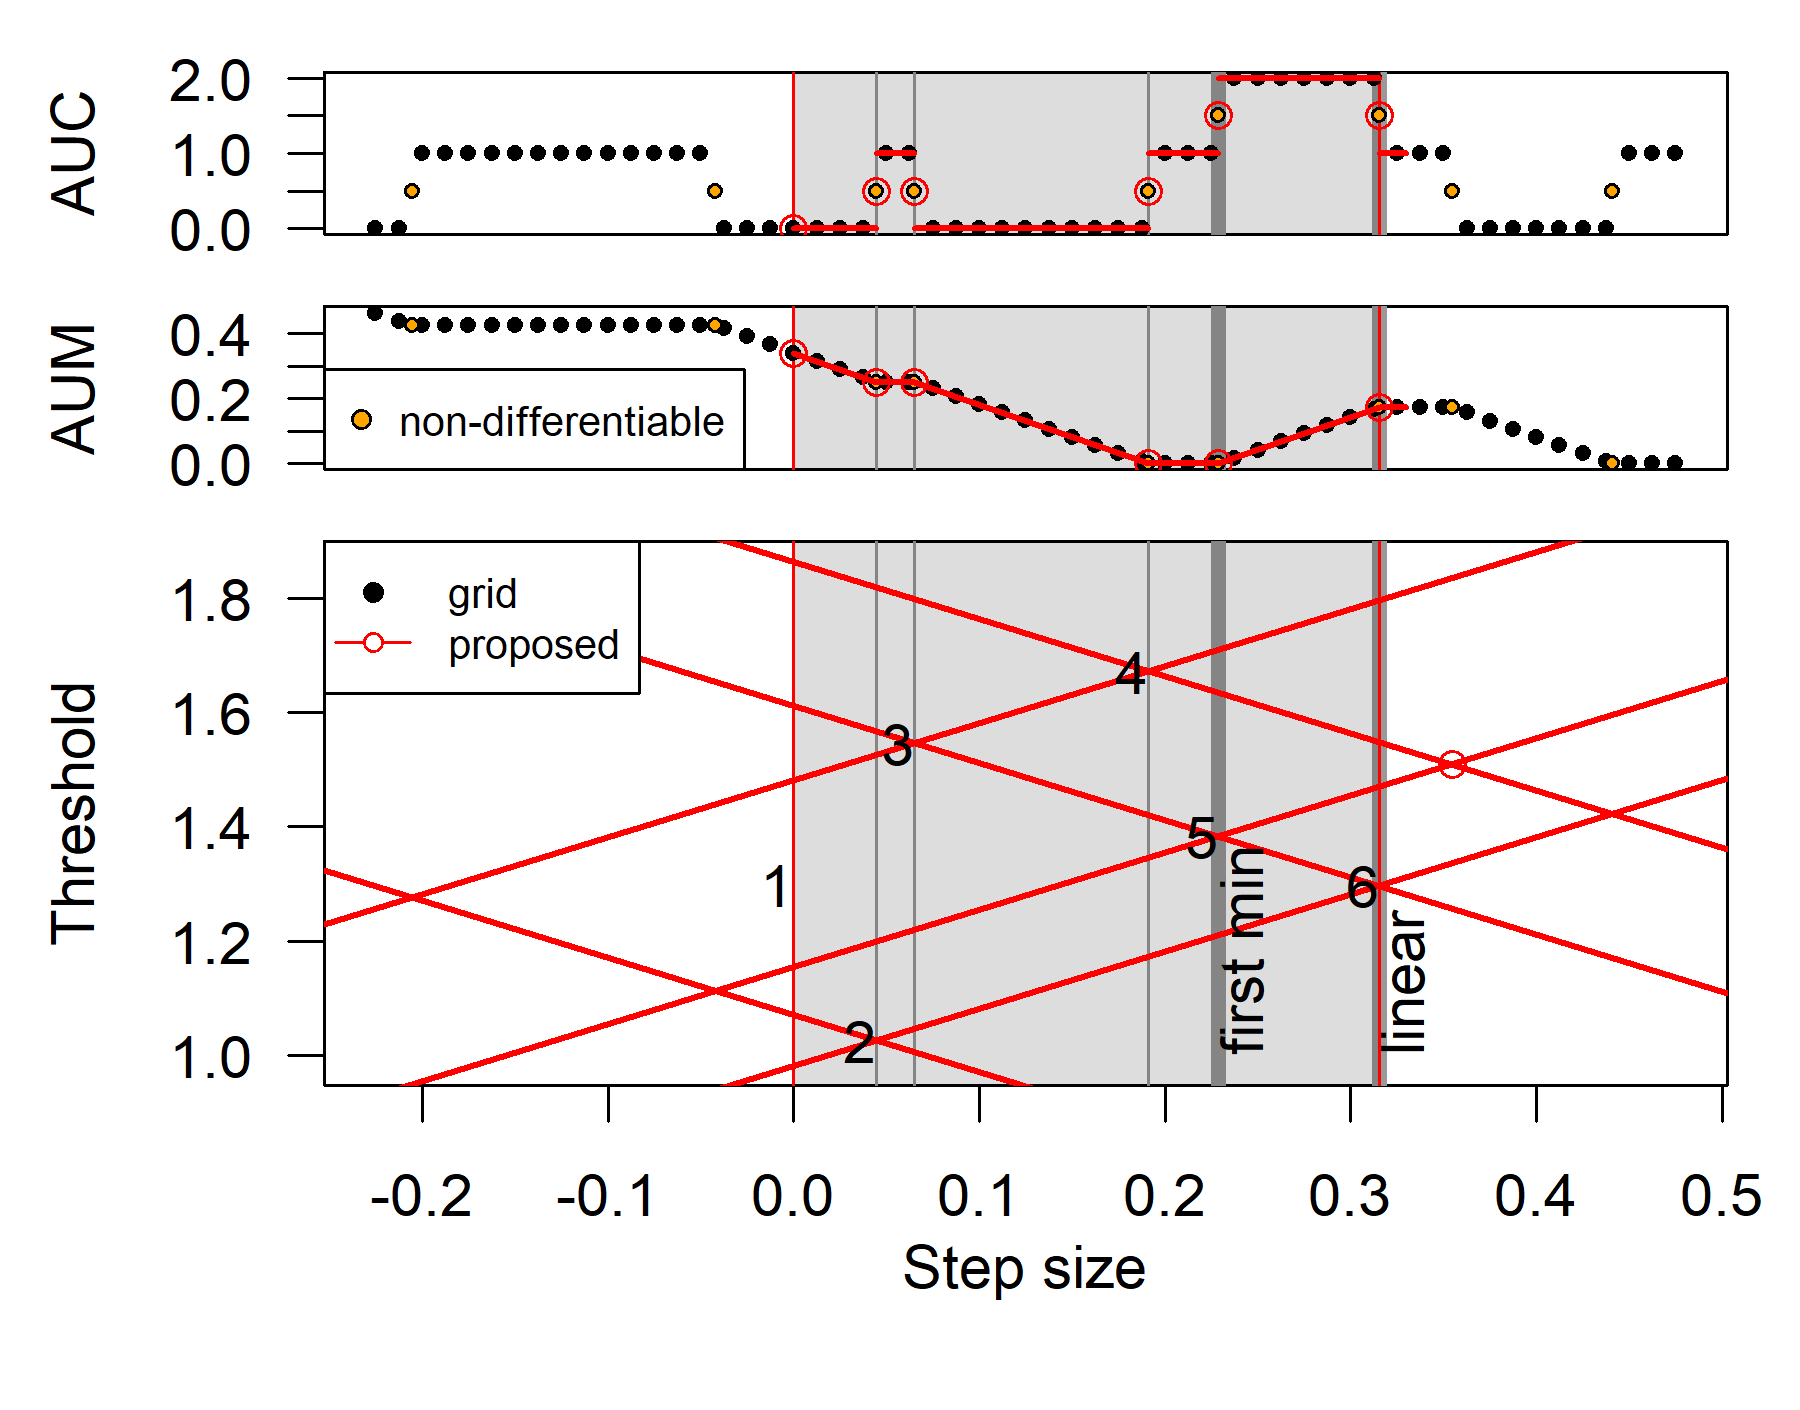
\includegraphics[width=\textwidth]{figure-line-search-example-6}
\end{frame}


\begin{frame}
  \frametitle{AUM/AUC line search, iteration 7}
  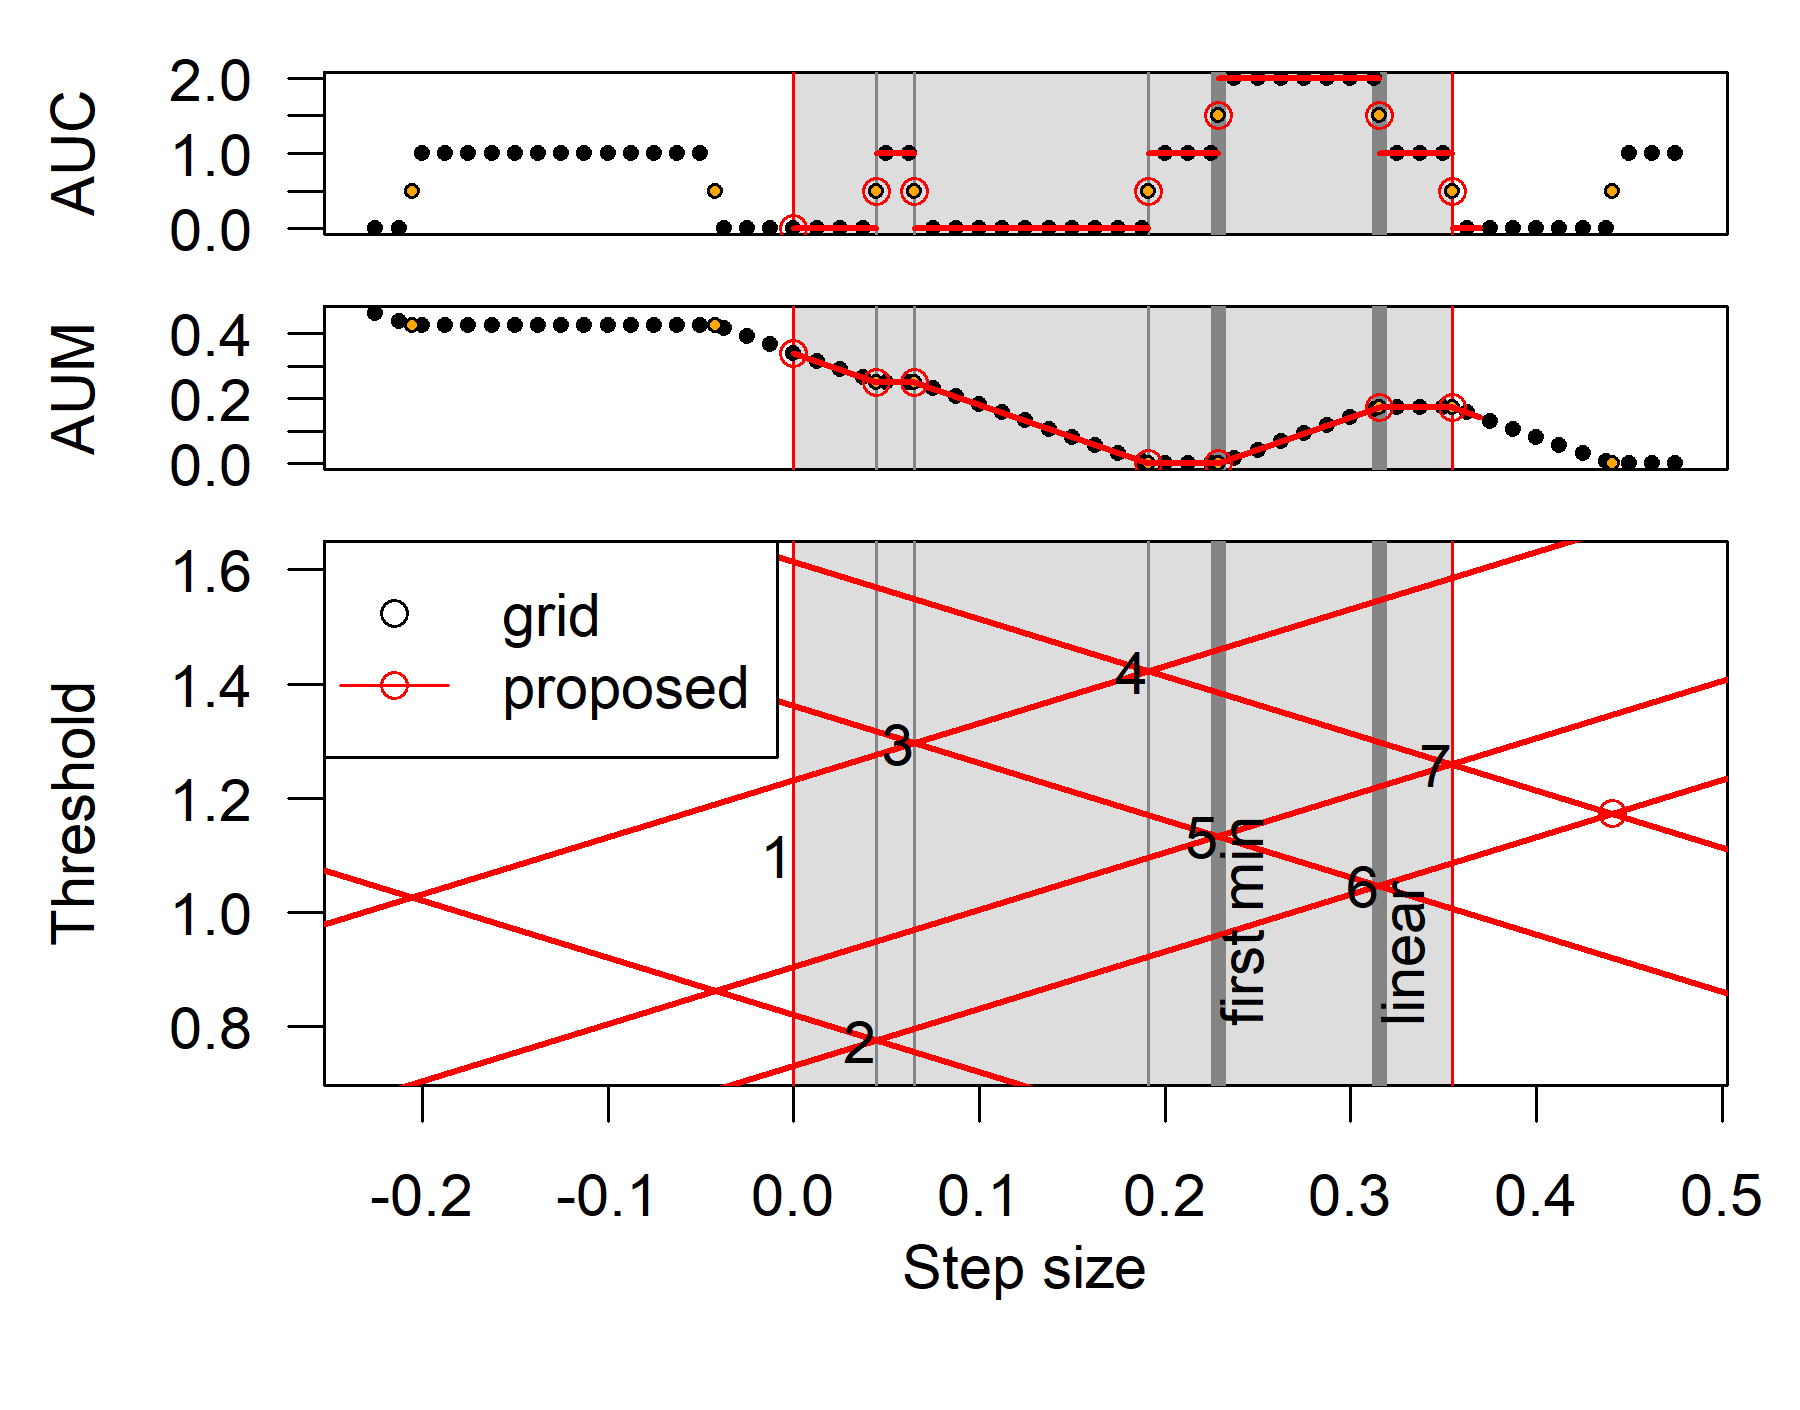
\includegraphics[width=\textwidth]{figure-line-search-example-7}
\end{frame}


\begin{frame}
  \frametitle{AUM/AUC line search, iteration 8}
  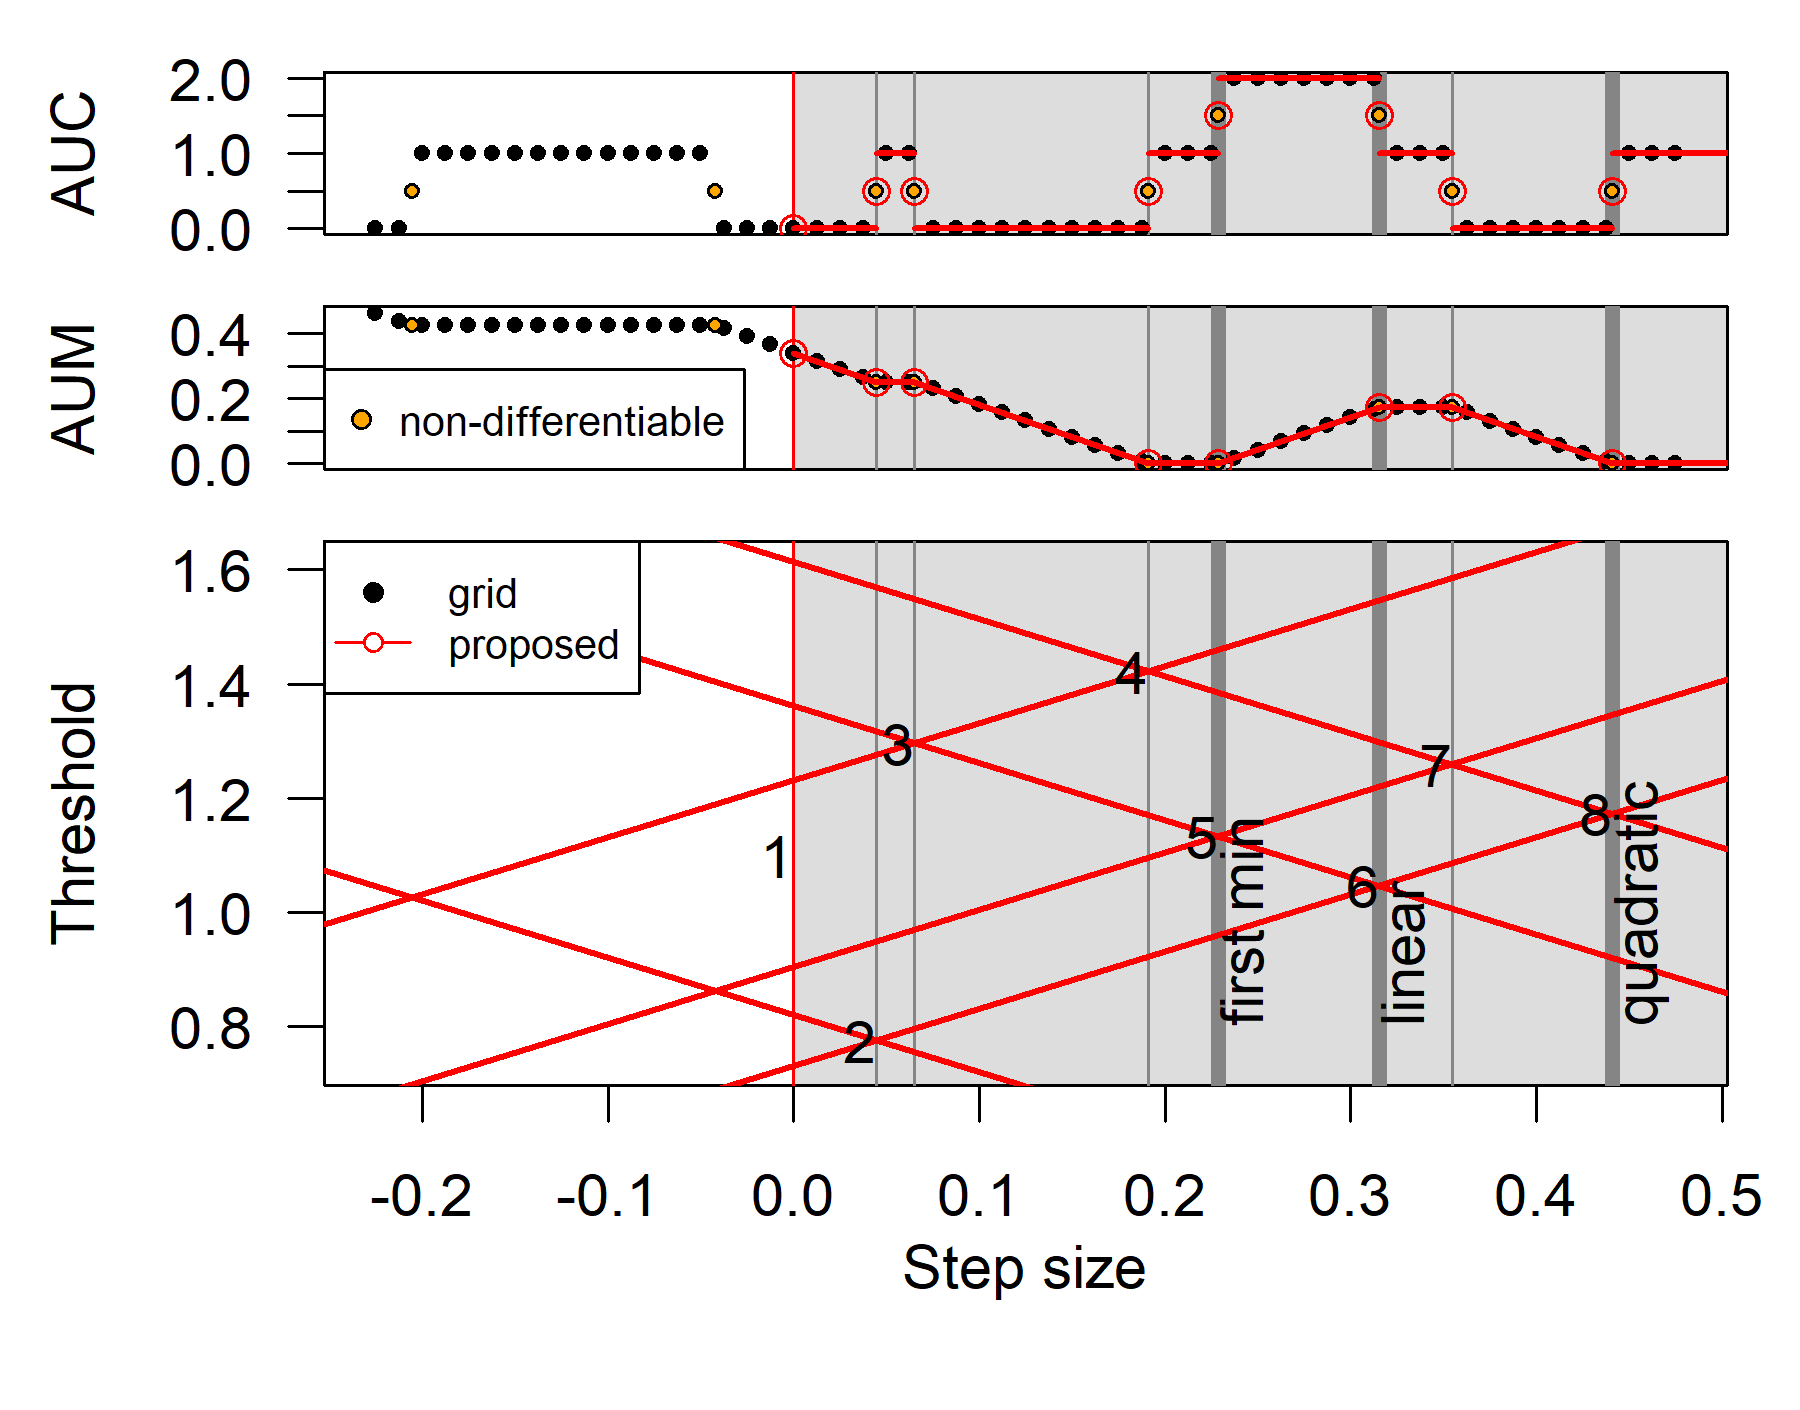
\includegraphics[width=\textwidth]{figure-line-search-example-8}
\end{frame}


\begin{frame}
  \frametitle{Complexity analysis of proposed algorithm}

  For $N$ labeled observations, input $N$ threshold line
  slope/intercept values. Possible next intersection points stored in
  a C++ STL map (red-black tree, sorted by step size), $O(\log N)$
  time insertion, $O(1)$ lookup of next intersection. Worst case $O(N)$
  space.
  %$O([N+I]\log N)$ time for $I$ iterations.
  \begin{description}
  \item[grid: standard grid search.] $O(G N\log N)$ time per step, 
    for $G$ grid points.
  \item[linear(proposed): only first $N$ intersections.]
    $O(N\log N)$ time per step, relatively small step sizes chosen,
    relatively large number of steps overall in gradient descent.
  \item[quadratic(proposed): all $O(N^2)$ intersections.]
    $O(N^2\log N)$ time per step, large step sizes, small number of
    steps.
  \item[first min(proposed): keep iterating until first AUM increase.]
    Same as quadratic in worst case, but may be faster on average (it
    was faster than both quadratic and linear for the example on the
    previous slide).
  \end{description}
\end{frame}

\section{Empirical results: increased speed and comparable accuracy using proposed complete line search} 

\begin{frame}
  \frametitle{Proposed search consistently faster than grid search}

  Analyzed supervised genomic change-point detection data set
  H3K4me3\_TDH\_immune ($N=1073$ to 1248)
%     > subtrain.sizes[data.name=="H3K4me3_TDH_immune"]
%             data.name      cv.type test.fold n.subtrain.diffs
% 1: H3K4me3_TDH_immune equal_labels         1             1248
% 2: H3K4me3_TDH_immune equal_labels         2             1200
% 3: H3K4me3_TDH_immune equal_labels         3             1197
% 4: H3K4me3_TDH_immune equal_labels         4             1073
  from UCI Machine Learning Repository,
  {\scriptsize \url{https://archive.ics.uci.edu/ml/datasets/chipseq},}
  Train/test splits defined via 4-fold CV, linear model initialized by
  minimizing regularized convex loss (surrogate for label error,
  Hocking \emph{et al.} ICML 2013), keep doing AUM rate gradient
  descent steps (with line search) until subtrain loss stops decreasing.

  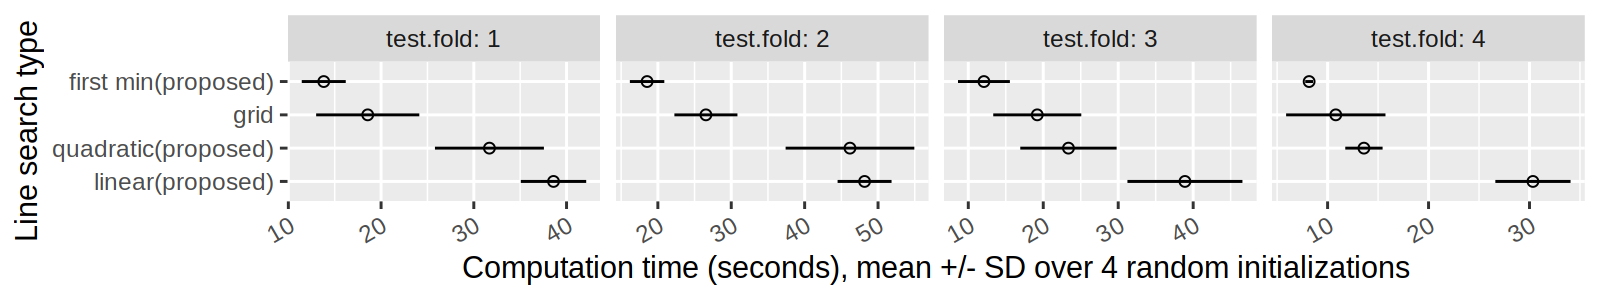
\includegraphics[width=\textwidth]{figure-line-search-complexity-compare-H3K4me3_TDH_immune-equal_labels-rate-IntervalRegressionCV-seconds}

  \begin{description}
  \item[first min(proposed):] keep iterating until first AUM
    increase.
  \item[grid:] search over step
    size$\in\{10^{-9},10^{-8},\dots,10^1,10^0\}$.
  \item[quadratic(proposed):] all line search iterations.
  \item[linear(proposed):] only first $N$ line search iterations.
  \end{description}
\end{frame}

\begin{frame}
  \frametitle{Proposed search has similar accuracy as grid search}

  Analyzed supervised genomic change-point detection data set
  H3K4me3\_TDH\_immune ($N=1073$ to 1248)
%     > subtrain.sizes[data.name=="H3K4me3_TDH_immune"]
%             data.name      cv.type test.fold n.subtrain.diffs
% 1: H3K4me3_TDH_immune equal_labels         1             1248
% 2: H3K4me3_TDH_immune equal_labels         2             1200
% 3: H3K4me3_TDH_immune equal_labels         3             1197
% 4: H3K4me3_TDH_immune equal_labels         4             1073
  from UCI Machine Learning Repository,
  {\scriptsize \url{https://archive.ics.uci.edu/ml/datasets/chipseq},}
  Train/test splits defined via 4-fold CV, linear model initialized by
  minimizing regularized convex loss (surrogate for label error,
  Hocking \emph{et al.} ICML 2013), keep doing AUM rate gradient
  descent steps (with line search) until subtrain loss stops decreasing.

  
\includegraphics[width=\textwidth]{figure-line-search-complexity-compare-H3K4me3_TDH_immune-equal_labels-rate-IntervalRegressionCV-initial}

  \begin{description}
  \item[first min(proposed):] keep iterating until first AUM
    increase.
  \item[grid:] search over step
    size$\in\{10^{-9},10^{-8},\dots,10^1,10^0\}$.
  \item[quadratic(proposed):] all line search iterations.
  \item[linear(proposed):] only first $N$ line search iterations.
  \end{description}
\end{frame}


\begin{frame}
  \frametitle{Asymptotic time complexity analysis}

  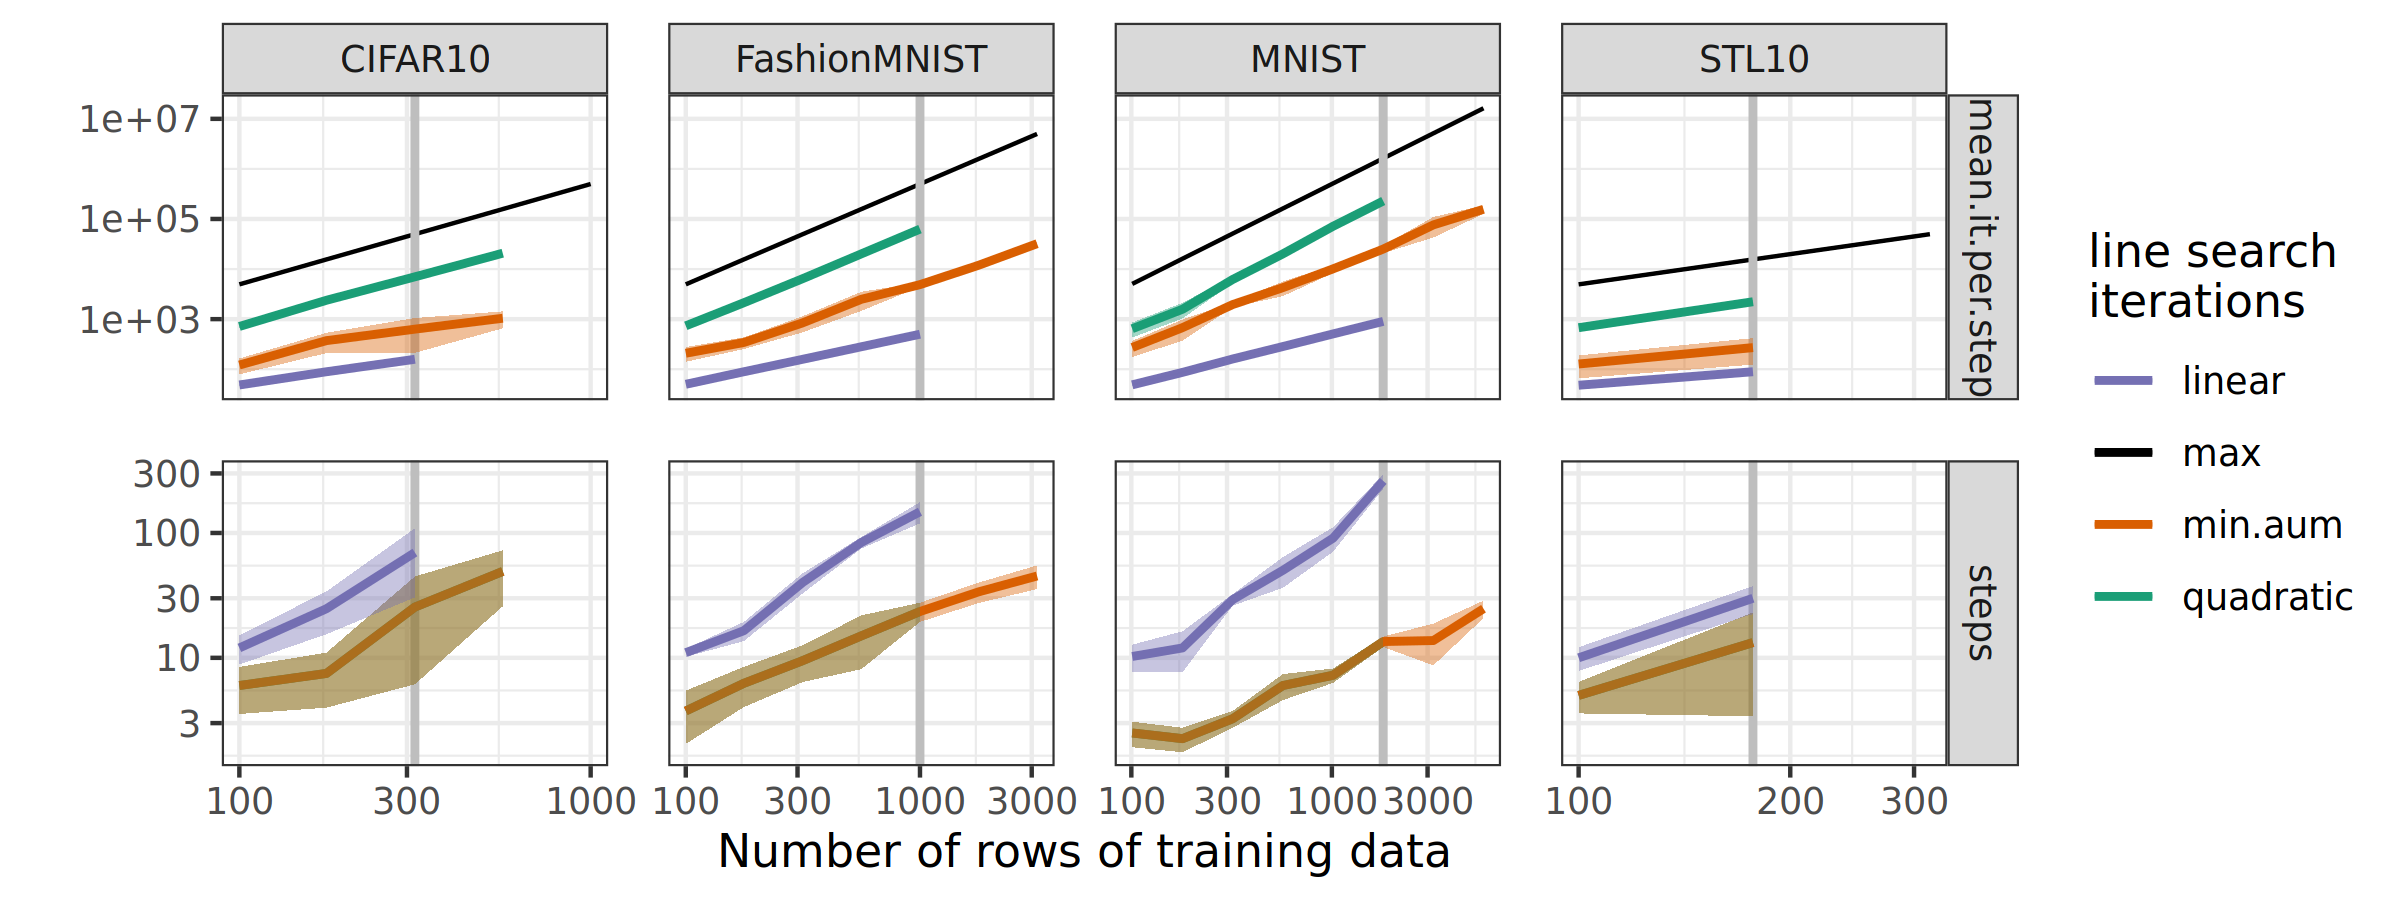
\includegraphics[width=\textwidth]{data_Classif_figure_units}

  \begin{description}
  \item[max:] theoretical worst case, $N(N-1)/2$ iterations.
  \item[quadratic(proposed):] all line search iterations.
  \item[first min(proposed):] keep iterating until first AUM increase
    (same number of steps/solution as quadratic, but asymptotically 
    faster/smaller slope).
  \item[linear(proposed):] only first $N$ line search iterations.    
  \end{description}
\end{frame}


\section{Discussion and Conclusions}

\begin{frame}
  \frametitle{Discussion and Conclusions}
  \begin{itemize}
  \item Area Under the ROC Curve (AUC) is used to evaluate binary
    classification and changepoint detection algorithms.
  % \item In changepoint detection there can be loops in ROC curves, so
  %   maximizing AUC greater than 1 is not be desirable.
  % \item In changepoint detection, maximizing Area Under ROC curve is
  %   non-trivial even for the train set with unconstrained
  %   predictions.
  \item Hocking, Hillman, \emph{Journal of Machine Learning Research}
    (2023), proposed AUM=Area Under Min(FP,FN), a new
    differentiable surrogate loss for AUC optimization.
  \item In this talk we proposed new gradient descent algorithms with
    efficient complete line search, for optimizing AUM/AUC.
  \item Empirical results provide evidence that proposed complete line
    search is consistently faster than grid search, and has 
    comparable accuracy (in terms of max validation AUC).
  \item Line search implemented in R/C++:
    {\scriptsize
    \url{https://cloud.r-project.org/web/packages/aum/} (R/C++ line search)
    }
  \item Future work: line search for non-linear prediction functions
    such as neural networks with ReLU activation?
  \end{itemize}
\end{frame}

\begin{frame}
  \frametitle{Thanks to co-author Jadon Fowler! (second from left)}

  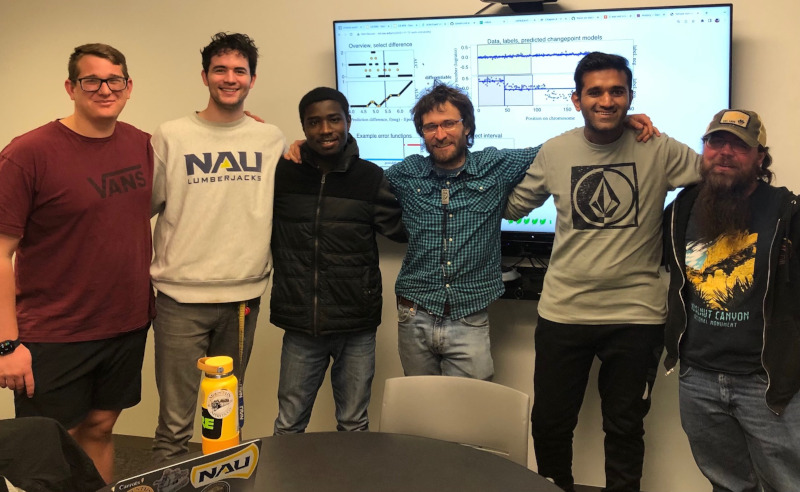
\includegraphics[height=3in]{2023-02-02-group-meeting}

  Contact: toby.hocking@nau.edu

\end{frame}

\begin{frame}
  \frametitle{AUC can be greater than one for change-point problems with non-monotonic error functions}
  \centering
  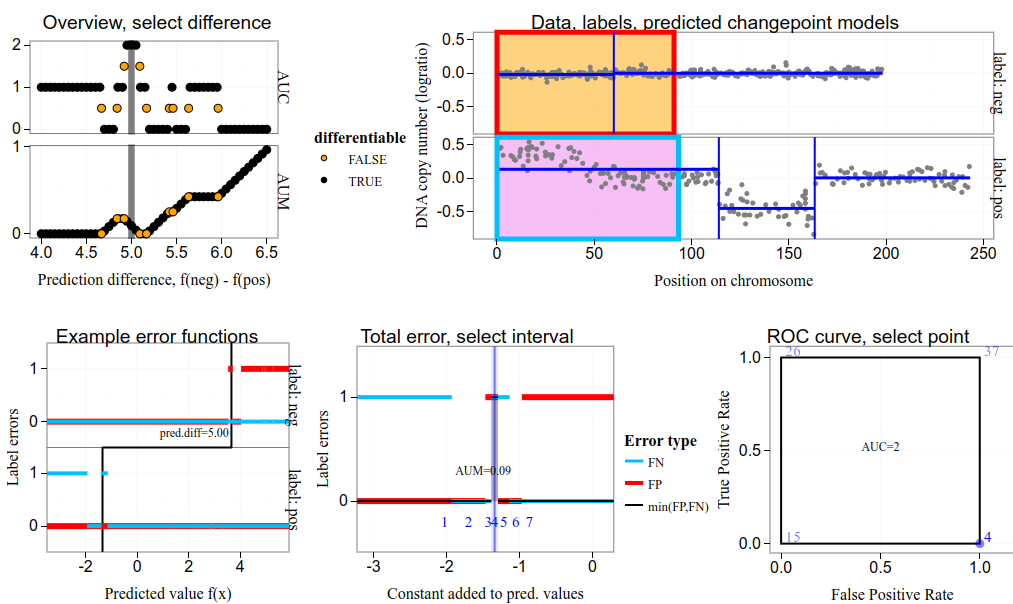
\includegraphics[height=0.7\textheight]{screenshot-auc-2-example}
  \scriptsize
  \url{https://nhintruong.github.io/figure-aum-convexity-interactive}
\end{frame}

\begin{frame}
  \frametitle{Initial/optimized AUC/AUM for change-point problems}
  \centering
  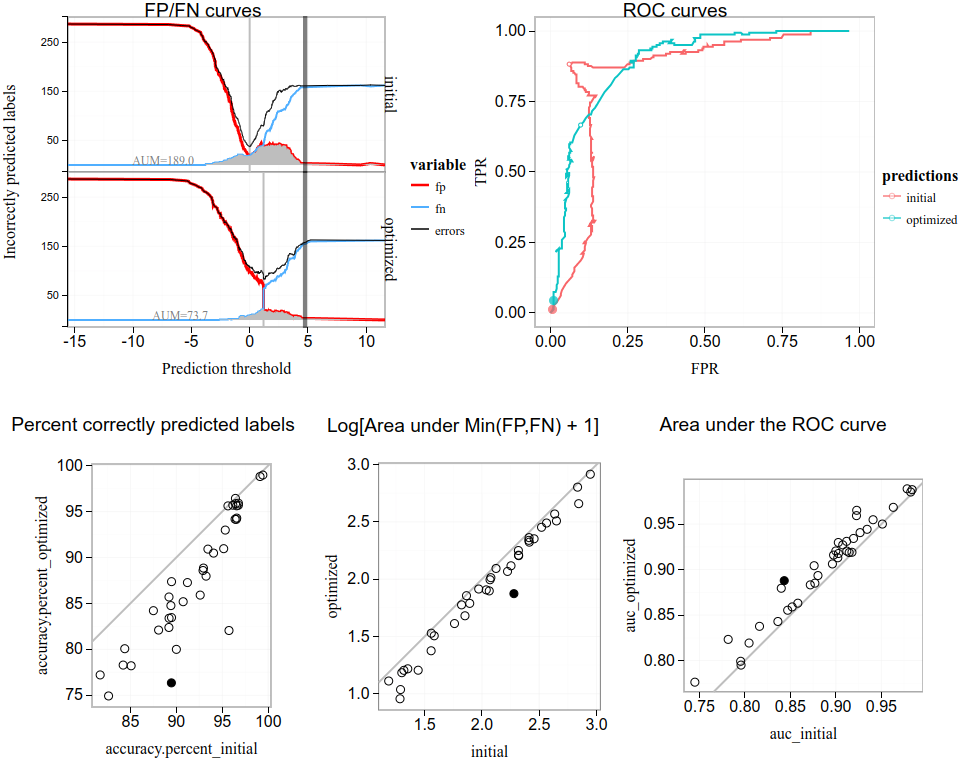
\includegraphics[height=0.7\textheight]{figure-auc-improved-interactive-screenshot}
  \url{https://tdhock.github.io/2023-11-21-auc-improved}
\end{frame}

\end{document}
